% lecture2_ro.tex -- GENERATED by build_L2.py from L2_numbers.json; do not edit by hand.
\documentclass[10pt,aspectratio=169,t]{beamer}
% =============================================================================
% emqa_preamble.tex -- shared Beamer preamble of Energy Markets Quantitative Analysis (EMQA)
% Used by every lecture: lectures/Lk/lecturek.tex does
%   \documentclass[10pt,aspectratio=169,t]{beamer}
%   % =============================================================================
% emqa_preamble.tex -- shared Beamer preamble of Energy Markets Quantitative Analysis (EMQA)
% Used by every lecture: lectures/Lk/lecturek.tex does
%   \documentclass[10pt,aspectratio=169,t]{beamer}
%   % =============================================================================
% emqa_preamble.tex -- shared Beamer preamble of Energy Markets Quantitative Analysis (EMQA)
% Used by every lecture: lectures/Lk/lecturek.tex does
%   \documentclass[10pt,aspectratio=169,t]{beamer}
%   \input{../common/emqa_preamble}
%   \emqalecture{k}{Lecture title}
% Logos live in lectures/common/logos/, charts in lectures/Lk/charts/.
% Do NOT add \hfuzz / \vfuzz / \hbadness here: overfull boxes must be fixed, not hidden.
% =============================================================================

\usetheme{default}
\setbeamersize{text margin left=7mm, text margin right=7mm}

% ---------------------------------------------------------------- packages
\usepackage[utf8]{inputenc}
\usepackage[T1]{fontenc}
\usepackage{lmodern}
\usepackage{amsmath, amssymb}
\usepackage{mathtools}
\usepackage{bm}
\usepackage{tikz}
\usetikzlibrary{arrows.meta, positioning, calc, shapes.misc}
\usepackage{booktabs}
\usepackage{array}
\usepackage{graphicx}
\usepackage{colortbl}
\usepackage{xcolor}
\usepackage{multicol}
\hypersetup{colorlinks=true, linkcolor=MainBlue, urlcolor=MainBlue, citecolor=MainBlue}
\graphicspath{{../common/logos/}}   % charts are included with their language folder: charts/en/, charts/ro/

% ---------------------------------------------------------------- colours
\definecolor{MainBlue}{RGB}{26, 58, 110}
\definecolor{IDAred}{RGB}{205, 0, 0}
\definecolor{DarkGray}{RGB}{51, 51, 51}
\definecolor{FooterGray}{RGB}{100, 100, 100}
\definecolor{BlockGray}{RGB}{236, 238, 242}
\definecolor{KeynoteGray}{RGB}{218, 218, 218}
\definecolor{Crimson}{RGB}{190, 40, 50}
\definecolor{Forest}{RGB}{30, 110, 50}
\definecolor{Bitter}{RGB}{214, 150, 20}
% chart palette (same hex values as lectures/common/emqa_plot.py)
\definecolor{SerRO}{HTML}{2A78D6}
\definecolor{SerDE}{HTML}{EB6834}
\definecolor{SerHU}{HTML}{1BAF7A}
\definecolor{SerBG}{HTML}{EDA100}

\setbeamertemplate{background}{%
  \begin{tikzpicture}[remember picture, overlay]
    \shade[shading=axis, shading angle=315, top color=white, bottom color=KeynoteGray]
      (current page.south west) rectangle (current page.north east);
  \end{tikzpicture}}
\setbeamercolor{background canvas}{bg=}
\setbeamercolor{structure}{fg=MainBlue}
\setbeamercolor{normal text}{fg=DarkGray}
\setbeamercolor{title}{fg=IDAred}
\setbeamercolor{frametitle}{fg=IDAred, bg=}
\setbeamercolor{block title}{bg=MainBlue, fg=white}
\setbeamercolor{block body}{bg=BlockGray, fg=DarkGray}
\setbeamercolor{block title alerted}{bg=Crimson, fg=white}
\setbeamercolor{block body alerted}{bg=Crimson!7, fg=DarkGray}
\setbeamercolor{block title example}{bg=Forest, fg=white}
\setbeamercolor{block body example}{bg=Forest!7, fg=DarkGray}
\setbeamercolor{item}{fg=MainBlue}
\setbeamerfont{frametitle}{size=\large, series=\bfseries}
\setbeamerfont{block title}{size=\small, series=\bfseries}
\setbeamertemplate{blocks}[rounded][shadow=false]
\setbeamertemplate{itemize item}{\color{MainBlue}$\boxdot$}
\setbeamertemplate{itemize subitem}{\color{MainBlue}\scriptsize$\blacktriangleright$}
% compact two-level lists: level 1 = main point, level 2 = details (no text outside bullets)
\setbeamerfont{itemize/enumerate subbody}{size=\footnotesize}
\setlength{\leftmargini}{1.1em}
\setlength{\leftmarginii}{1.1em}
\setbeamertemplate{itemize/enumerate body begin}{\setlength{\topsep}{0pt}\setlength{\partopsep}{0pt}\setlength{\parskip}{0pt}}
\setbeamertemplate{itemize/enumerate subbody begin}{\setlength{\topsep}{0pt}\setlength{\partopsep}{0pt}\setlength{\itemsep}{0pt}\vspace{-0.4ex}}

\setbeamertemplate{enumerate item}{\color{MainBlue}\insertenumlabel.}
\setlength{\leftmargini}{1.3em}
\setlength{\leftmarginii}{1.2em}
\setbeamertemplate{navigation symbols}{}
\setbeamertemplate{section in toc}{\color{MainBlue}$\blacktriangleright$~\inserttocsection}
\setbeamertemplate{caption}{\raggedright\insertcaption\par}
% frame subtitle = precise citation line under the claim title (Weron style)
\setbeamerfont{framesubtitle}{size=\footnotesize}
\setbeamercolor{framesubtitle}{fg=FooterGray}
% outline that reappears at every section with the current section highlighted
\setbeamertemplate{section in toc shaded}[default][35]
\setbeamertemplate{subsection in toc shaded}[default][35]
\setbeamertemplate{subsection in toc}{\leavevmode\leftskip=2.2em\color{DarkGray}\small\inserttocsubsection\par}
\AtBeginSection[]{{\begin{frame}{\txtoutline}\vspace{2mm}\small
  \tableofcontents[currentsection,hideothersubsections]\end{frame}}}

% ---------------------------------------------------------------- head and foot
\setbeamertemplate{headline}{%
  \vskip10pt%
  \hbox to \paperwidth{\hskip0.5cm%
    {\small\color{FooterGray}\renewcommand{\hyperlink}[2]{##2}\insertsectionhead}%
    \hfill\textcolor{FooterGray}{\small\insertframenumber}\hskip0.5cm}%
  \vskip4pt{\color{FooterGray}\hrule height 0.4pt}}
% footer as in the other courses (MFM, SFM): course name on the left, small sparkline on the right
\setbeamertemplate{footline}{%
  {\color{FooterGray}\hrule height 0.4pt}\vskip4pt%
  \hbox to \paperwidth{\hskip0.5cm%
    \textcolor{FooterGray}{\small\txtcourse}%
    \hfill\raisebox{-0.1em}{\begin{tikzpicture}[x=0.08em, y=0.08em, line width=0.4pt]
      \draw[FooterGray] (0,3) -- (1,4) -- (2,3.5) -- (3,5) -- (4,4) -- (5,6) -- (6,5.5) -- (7,4) -- (8,5) -- (9,7) -- (10,6) -- (11,5) -- (12,6.5) -- (13,8) -- (14,7) -- (15,6) -- (16,7.5) -- (17,9) -- (18,8) -- (19,7) -- (20,8.5) -- (21,10) -- (22,9) -- (23,8) -- (24,9.5);
    \end{tikzpicture}}\hskip0.5cm}%
  \vskip6pt}

% ---------------------------------------------------------------- title page
\defbeamertemplate*{title page}{emqa}[1][]{%
  \vspace{0.15cm}
  \begin{center}
    \href{https://www.ase.ro}{
\includegraphics[height=0.9cm]{ase_logo.png}}\hspace{0.3cm}%
    \href{https://ipe.ro/new}{
\includegraphics[height=0.9cm]{acad_logo.png}}\hspace{0.3cm}%
    \href{https://theida.net}{
\includegraphics[height=0.9cm]{ida_logo.png}}\hspace{0.3cm}%
    \href{https://blockchain-research-center.com}{
\includegraphics[height=0.9cm]{brc_logo.png}}\hspace{0.3cm}%
    \href{https://www.ai4efin.ase.ro}{
\includegraphics[height=0.9cm]{ai4efin_logo.png}}\hspace{0.3cm}%
    \href{https://www.digital-finance-msca.com}{
\includegraphics[height=0.9cm]{msca_logo.png}}%
  \end{center}
  \vspace{0.45cm}
  \begin{center}
    \begin{minipage}{0.1\textwidth}\centering
      \href{https://quantlet.com}{
\includegraphics[height=0.9cm]{ql_logo.png}}\end{minipage}%
    \begin{minipage}{0.78\textwidth}\centering
      {\Large\bfseries\usebeamercolor[fg]{title}\inserttitle}\par\vspace{0.25cm}
      {\large\usebeamercolor[fg]{title}\insertsubtitle}\end{minipage}%
    \begin{minipage}{0.1\textwidth}\centering
      \href{https://quantinar.com}{
\includegraphics[height=0.9cm]{qr_logo.png}}\end{minipage}
  \end{center}
  \vfill
  \hspace{0.4cm}{\bfseries\insertauthor}\par\vspace{0.12cm}
  \hspace{0.4cm}\begin{minipage}[t]{0.92\textwidth}\raggedright\footnotesize\insertinstitute\end{minipage}
  \par\vspace{0.4cm}}

% ---------------------------------------------------------------- lecture metadata
\newcommand{\emqashort}{}
\newcommand{\emqanb}{notebooks}
\newcommand{\emqarepo}{https://github.com/danpele/EMQA/tree/main}
% language-dependent labels (English default; \emqaromanian switches to Romanian, call it before \emqalecture)
\newcommand{\txtcourse}{Energy Markets Quantitative Analysis}
\newcommand{\txtlecture}{Lecture}
\newcommand{\txtoutline}{Outline}
\newcommand{\txtintuition}{In one sentence:}
\newcommand{\txtjob}{In practice:}
\newcommand{\txttry}{Experiment yourself:}
\newcommand{\txtwhere}{where}
\newcommand{\txtsim}{SIMULATED DATA (teaching illustration)}
\newcommand{\txtnbsuffix}{}
\newcommand{\txtinstitute}{Bucharest University of Economic Studies, Department of Statistics and Econometrics\\
    Romanian Academy, Institute for Economic Forecasting\\
    IDA Institute Digital Assets \textbullet\ AI4EFin \textbullet\ MSCA Digital Finance}
\newcommand{\emqaromanian}{%
  \renewcommand{\txtcourse}{Analiza cantitativă a piețelor de energie}%
  \renewcommand{\txtlecture}{Cursul}%
  \renewcommand{\txtoutline}{Cuprins}%
  \renewcommand{\txtintuition}{Pe scurt:}%
  \renewcommand{\txtjob}{În practică:}%
  \renewcommand{\txttry}{Exercițiu practic:}%
  \renewcommand{\txtwhere}{unde}%
  \renewcommand{\txtsim}{DATE SIMULATE (doar pentru ilustrare)}%
  \renewcommand{\txtnbsuffix}{\string_ro}%
  \renewcommand{\txtinstitute}{Academia de Studii Economice din București, Departamentul de Statistică și Econometrie\\
    Academia Română, Institutul de Prognoză Economică\\
    IDA Institute Digital Assets \textbullet\ AI4EFin \textbullet\ MSCA Digital Finance}}
\newcommand{\emqalecture}[2]{%
  \renewcommand{\emqashort}{\txtlecture\ #1}%
  \renewcommand{\emqanb}{notebooks/L#1\string_notebook\txtnbsuffix.ipynb}%
  \title[EMQA]{\txtcourse}%
  \subtitle{\txtlecture\ #1: #2}%
  \author{Prof.\ dr.\ Daniel Traian PELE}%
  \institute{\txtinstitute}%
  \date{}}

% ---------------------------------------------------------------- teaching blocks (MBA clarity rule)
% \intuition{one plain sentence}  ->  formula with every symbol defined  ->  real-data example  ->  \manager{one line}
\newcommand{\intuition}[1]{\begin{itemize}\item {\color{MainBlue}\textbf{\txtintuition}}~#1\end{itemize}\vspace{0.6mm}}
\newcommand{\manager}[1]{\colorbox{Forest!10}{\parbox{\dimexpr\linewidth-2\fboxsep\relax}{\footnotesize
  \begin{itemize}\setlength{\itemsep}{0pt}\item \textbf{\color{Forest}\txtjob}~#1\end{itemize}}}}
% Experiment yourself: pointer to the matching notebook section
\newcommand{\tryit}[1]{{\scriptsize\href{\emqarepo/\emqanb}{%
  \raisebox{-0.15em}{
\includegraphics[height=0.85em]{ql_logo.png}}\,\textbf{\txttry}~\color{MainBlue}#1}}}
% bottom row: manager line (left) + experiment pointer (right), pinned to the bottom of the frame
\newcommand{\bottomrow}[2]{\par\vfill\noindent\begin{minipage}[b]{0.72\linewidth}#1\end{minipage}\hfill
  \begin{minipage}[b]{0.26\linewidth}\raggedleft #2\end{minipage}\par\vspace{0.5mm}}
\newcommand{\where}[1]{{\footnotesize\textbf{\txtwhere}~#1\par}}

% ---------------------------------------------------------------- helpers
% chart source line under a figure: \chartsource{Source ...; period ...}
\newcommand{\chartsource}[1]{\par\vspace{1pt}{\scriptsize\color{FooterGray}#1\par}}
% link to code: \quantlet{label}{path inside the repo}
\newcommand{\quantlet}[2]{\par\vspace{1pt}\hfill\href{\emqarepo/#2}{%
  \raisebox{-0.15em}{
\includegraphics[height=0.75em]{ql_logo.png}}\textcolor{MainBlue}{\scriptsize\ #1}}}
\newcommand{\simlabel}{\colorbox{Crimson!12}{\scriptsize\bfseries\color{Crimson}\txtsim}}
\newcommand{\E}{\mathbb{E}}
\newcommand{\Var}{\operatorname{Var}}
\newcommand{\Cov}{\operatorname{Cov}}
\newcommand{\Corr}{\operatorname{Corr}}
\newcommand{\asinh}{\operatorname{asinh}}
\newcommand{\iid}{\overset{\text{i.i.d.}}{\sim}}
\newcommand{\EUR}{EUR}

%   \emqalecture{k}{Lecture title}
% Logos live in lectures/common/logos/, charts in lectures/Lk/charts/.
% Do NOT add \hfuzz / \vfuzz / \hbadness here: overfull boxes must be fixed, not hidden.
% =============================================================================

\usetheme{default}
\setbeamersize{text margin left=7mm, text margin right=7mm}

% ---------------------------------------------------------------- packages
\usepackage[utf8]{inputenc}
\usepackage[T1]{fontenc}
\usepackage{lmodern}
\usepackage{amsmath, amssymb}
\usepackage{mathtools}
\usepackage{bm}
\usepackage{tikz}
\usetikzlibrary{arrows.meta, positioning, calc, shapes.misc}
\usepackage{booktabs}
\usepackage{array}
\usepackage{graphicx}
\usepackage{colortbl}
\usepackage{xcolor}
\usepackage{multicol}
\hypersetup{colorlinks=true, linkcolor=MainBlue, urlcolor=MainBlue, citecolor=MainBlue}
\graphicspath{{../common/logos/}}   % charts are included with their language folder: charts/en/, charts/ro/

% ---------------------------------------------------------------- colours
\definecolor{MainBlue}{RGB}{26, 58, 110}
\definecolor{IDAred}{RGB}{205, 0, 0}
\definecolor{DarkGray}{RGB}{51, 51, 51}
\definecolor{FooterGray}{RGB}{100, 100, 100}
\definecolor{BlockGray}{RGB}{236, 238, 242}
\definecolor{KeynoteGray}{RGB}{218, 218, 218}
\definecolor{Crimson}{RGB}{190, 40, 50}
\definecolor{Forest}{RGB}{30, 110, 50}
\definecolor{Bitter}{RGB}{214, 150, 20}
% chart palette (same hex values as lectures/common/emqa_plot.py)
\definecolor{SerRO}{HTML}{2A78D6}
\definecolor{SerDE}{HTML}{EB6834}
\definecolor{SerHU}{HTML}{1BAF7A}
\definecolor{SerBG}{HTML}{EDA100}

\setbeamertemplate{background}{%
  \begin{tikzpicture}[remember picture, overlay]
    \shade[shading=axis, shading angle=315, top color=white, bottom color=KeynoteGray]
      (current page.south west) rectangle (current page.north east);
  \end{tikzpicture}}
\setbeamercolor{background canvas}{bg=}
\setbeamercolor{structure}{fg=MainBlue}
\setbeamercolor{normal text}{fg=DarkGray}
\setbeamercolor{title}{fg=IDAred}
\setbeamercolor{frametitle}{fg=IDAred, bg=}
\setbeamercolor{block title}{bg=MainBlue, fg=white}
\setbeamercolor{block body}{bg=BlockGray, fg=DarkGray}
\setbeamercolor{block title alerted}{bg=Crimson, fg=white}
\setbeamercolor{block body alerted}{bg=Crimson!7, fg=DarkGray}
\setbeamercolor{block title example}{bg=Forest, fg=white}
\setbeamercolor{block body example}{bg=Forest!7, fg=DarkGray}
\setbeamercolor{item}{fg=MainBlue}
\setbeamerfont{frametitle}{size=\large, series=\bfseries}
\setbeamerfont{block title}{size=\small, series=\bfseries}
\setbeamertemplate{blocks}[rounded][shadow=false]
\setbeamertemplate{itemize item}{\color{MainBlue}$\boxdot$}
\setbeamertemplate{itemize subitem}{\color{MainBlue}\scriptsize$\blacktriangleright$}
% compact two-level lists: level 1 = main point, level 2 = details (no text outside bullets)
\setbeamerfont{itemize/enumerate subbody}{size=\footnotesize}
\setlength{\leftmargini}{1.1em}
\setlength{\leftmarginii}{1.1em}
\setbeamertemplate{itemize/enumerate body begin}{\setlength{\topsep}{0pt}\setlength{\partopsep}{0pt}\setlength{\parskip}{0pt}}
\setbeamertemplate{itemize/enumerate subbody begin}{\setlength{\topsep}{0pt}\setlength{\partopsep}{0pt}\setlength{\itemsep}{0pt}\vspace{-0.4ex}}

\setbeamertemplate{enumerate item}{\color{MainBlue}\insertenumlabel.}
\setlength{\leftmargini}{1.3em}
\setlength{\leftmarginii}{1.2em}
\setbeamertemplate{navigation symbols}{}
\setbeamertemplate{section in toc}{\color{MainBlue}$\blacktriangleright$~\inserttocsection}
\setbeamertemplate{caption}{\raggedright\insertcaption\par}
% frame subtitle = precise citation line under the claim title (Weron style)
\setbeamerfont{framesubtitle}{size=\footnotesize}
\setbeamercolor{framesubtitle}{fg=FooterGray}
% outline that reappears at every section with the current section highlighted
\setbeamertemplate{section in toc shaded}[default][35]
\setbeamertemplate{subsection in toc shaded}[default][35]
\setbeamertemplate{subsection in toc}{\leavevmode\leftskip=2.2em\color{DarkGray}\small\inserttocsubsection\par}
\AtBeginSection[]{{\begin{frame}{\txtoutline}\vspace{2mm}\small
  \tableofcontents[currentsection,hideothersubsections]\end{frame}}}

% ---------------------------------------------------------------- head and foot
\setbeamertemplate{headline}{%
  \vskip10pt%
  \hbox to \paperwidth{\hskip0.5cm%
    {\small\color{FooterGray}\renewcommand{\hyperlink}[2]{##2}\insertsectionhead}%
    \hfill\textcolor{FooterGray}{\small\insertframenumber}\hskip0.5cm}%
  \vskip4pt{\color{FooterGray}\hrule height 0.4pt}}
% footer as in the other courses (MFM, SFM): course name on the left, small sparkline on the right
\setbeamertemplate{footline}{%
  {\color{FooterGray}\hrule height 0.4pt}\vskip4pt%
  \hbox to \paperwidth{\hskip0.5cm%
    \textcolor{FooterGray}{\small\txtcourse}%
    \hfill\raisebox{-0.1em}{\begin{tikzpicture}[x=0.08em, y=0.08em, line width=0.4pt]
      \draw[FooterGray] (0,3) -- (1,4) -- (2,3.5) -- (3,5) -- (4,4) -- (5,6) -- (6,5.5) -- (7,4) -- (8,5) -- (9,7) -- (10,6) -- (11,5) -- (12,6.5) -- (13,8) -- (14,7) -- (15,6) -- (16,7.5) -- (17,9) -- (18,8) -- (19,7) -- (20,8.5) -- (21,10) -- (22,9) -- (23,8) -- (24,9.5);
    \end{tikzpicture}}\hskip0.5cm}%
  \vskip6pt}

% ---------------------------------------------------------------- title page
\defbeamertemplate*{title page}{emqa}[1][]{%
  \vspace{0.15cm}
  \begin{center}
    \href{https://www.ase.ro}{
\includegraphics[height=0.9cm]{ase_logo.png}}\hspace{0.3cm}%
    \href{https://ipe.ro/new}{
\includegraphics[height=0.9cm]{acad_logo.png}}\hspace{0.3cm}%
    \href{https://theida.net}{
\includegraphics[height=0.9cm]{ida_logo.png}}\hspace{0.3cm}%
    \href{https://blockchain-research-center.com}{
\includegraphics[height=0.9cm]{brc_logo.png}}\hspace{0.3cm}%
    \href{https://www.ai4efin.ase.ro}{
\includegraphics[height=0.9cm]{ai4efin_logo.png}}\hspace{0.3cm}%
    \href{https://www.digital-finance-msca.com}{
\includegraphics[height=0.9cm]{msca_logo.png}}%
  \end{center}
  \vspace{0.45cm}
  \begin{center}
    \begin{minipage}{0.1\textwidth}\centering
      \href{https://quantlet.com}{
\includegraphics[height=0.9cm]{ql_logo.png}}\end{minipage}%
    \begin{minipage}{0.78\textwidth}\centering
      {\Large\bfseries\usebeamercolor[fg]{title}\inserttitle}\par\vspace{0.25cm}
      {\large\usebeamercolor[fg]{title}\insertsubtitle}\end{minipage}%
    \begin{minipage}{0.1\textwidth}\centering
      \href{https://quantinar.com}{
\includegraphics[height=0.9cm]{qr_logo.png}}\end{minipage}
  \end{center}
  \vfill
  \hspace{0.4cm}{\bfseries\insertauthor}\par\vspace{0.12cm}
  \hspace{0.4cm}\begin{minipage}[t]{0.92\textwidth}\raggedright\footnotesize\insertinstitute\end{minipage}
  \par\vspace{0.4cm}}

% ---------------------------------------------------------------- lecture metadata
\newcommand{\emqashort}{}
\newcommand{\emqanb}{notebooks}
\newcommand{\emqarepo}{https://github.com/danpele/EMQA/tree/main}
% language-dependent labels (English default; \emqaromanian switches to Romanian, call it before \emqalecture)
\newcommand{\txtcourse}{Energy Markets Quantitative Analysis}
\newcommand{\txtlecture}{Lecture}
\newcommand{\txtoutline}{Outline}
\newcommand{\txtintuition}{In one sentence:}
\newcommand{\txtjob}{In practice:}
\newcommand{\txttry}{Experiment yourself:}
\newcommand{\txtwhere}{where}
\newcommand{\txtsim}{SIMULATED DATA (teaching illustration)}
\newcommand{\txtnbsuffix}{}
\newcommand{\txtinstitute}{Bucharest University of Economic Studies, Department of Statistics and Econometrics\\
    Romanian Academy, Institute for Economic Forecasting\\
    IDA Institute Digital Assets \textbullet\ AI4EFin \textbullet\ MSCA Digital Finance}
\newcommand{\emqaromanian}{%
  \renewcommand{\txtcourse}{Analiza cantitativă a piețelor de energie}%
  \renewcommand{\txtlecture}{Cursul}%
  \renewcommand{\txtoutline}{Cuprins}%
  \renewcommand{\txtintuition}{Pe scurt:}%
  \renewcommand{\txtjob}{În practică:}%
  \renewcommand{\txttry}{Exercițiu practic:}%
  \renewcommand{\txtwhere}{unde}%
  \renewcommand{\txtsim}{DATE SIMULATE (doar pentru ilustrare)}%
  \renewcommand{\txtnbsuffix}{\string_ro}%
  \renewcommand{\txtinstitute}{Academia de Studii Economice din București, Departamentul de Statistică și Econometrie\\
    Academia Română, Institutul de Prognoză Economică\\
    IDA Institute Digital Assets \textbullet\ AI4EFin \textbullet\ MSCA Digital Finance}}
\newcommand{\emqalecture}[2]{%
  \renewcommand{\emqashort}{\txtlecture\ #1}%
  \renewcommand{\emqanb}{notebooks/L#1\string_notebook\txtnbsuffix.ipynb}%
  \title[EMQA]{\txtcourse}%
  \subtitle{\txtlecture\ #1: #2}%
  \author{Prof.\ dr.\ Daniel Traian PELE}%
  \institute{\txtinstitute}%
  \date{}}

% ---------------------------------------------------------------- teaching blocks (MBA clarity rule)
% \intuition{one plain sentence}  ->  formula with every symbol defined  ->  real-data example  ->  \manager{one line}
\newcommand{\intuition}[1]{\begin{itemize}\item {\color{MainBlue}\textbf{\txtintuition}}~#1\end{itemize}\vspace{0.6mm}}
\newcommand{\manager}[1]{\colorbox{Forest!10}{\parbox{\dimexpr\linewidth-2\fboxsep\relax}{\footnotesize
  \begin{itemize}\setlength{\itemsep}{0pt}\item \textbf{\color{Forest}\txtjob}~#1\end{itemize}}}}
% Experiment yourself: pointer to the matching notebook section
\newcommand{\tryit}[1]{{\scriptsize\href{\emqarepo/\emqanb}{%
  \raisebox{-0.15em}{
\includegraphics[height=0.85em]{ql_logo.png}}\,\textbf{\txttry}~\color{MainBlue}#1}}}
% bottom row: manager line (left) + experiment pointer (right), pinned to the bottom of the frame
\newcommand{\bottomrow}[2]{\par\vfill\noindent\begin{minipage}[b]{0.72\linewidth}#1\end{minipage}\hfill
  \begin{minipage}[b]{0.26\linewidth}\raggedleft #2\end{minipage}\par\vspace{0.5mm}}
\newcommand{\where}[1]{{\footnotesize\textbf{\txtwhere}~#1\par}}

% ---------------------------------------------------------------- helpers
% chart source line under a figure: \chartsource{Source ...; period ...}
\newcommand{\chartsource}[1]{\par\vspace{1pt}{\scriptsize\color{FooterGray}#1\par}}
% link to code: \quantlet{label}{path inside the repo}
\newcommand{\quantlet}[2]{\par\vspace{1pt}\hfill\href{\emqarepo/#2}{%
  \raisebox{-0.15em}{
\includegraphics[height=0.75em]{ql_logo.png}}\textcolor{MainBlue}{\scriptsize\ #1}}}
\newcommand{\simlabel}{\colorbox{Crimson!12}{\scriptsize\bfseries\color{Crimson}\txtsim}}
\newcommand{\E}{\mathbb{E}}
\newcommand{\Var}{\operatorname{Var}}
\newcommand{\Cov}{\operatorname{Cov}}
\newcommand{\Corr}{\operatorname{Corr}}
\newcommand{\asinh}{\operatorname{asinh}}
\newcommand{\iid}{\overset{\text{i.i.d.}}{\sim}}
\newcommand{\EUR}{EUR}

%   \emqalecture{k}{Lecture title}
% Logos live in lectures/common/logos/, charts in lectures/Lk/charts/.
% Do NOT add \hfuzz / \vfuzz / \hbadness here: overfull boxes must be fixed, not hidden.
% =============================================================================

\usetheme{default}
\setbeamersize{text margin left=7mm, text margin right=7mm}

% ---------------------------------------------------------------- packages
\usepackage[utf8]{inputenc}
\usepackage[T1]{fontenc}
\usepackage{lmodern}
\usepackage{amsmath, amssymb}
\usepackage{mathtools}
\usepackage{bm}
\usepackage{tikz}
\usetikzlibrary{arrows.meta, positioning, calc, shapes.misc}
\usepackage{booktabs}
\usepackage{array}
\usepackage{graphicx}
\usepackage{colortbl}
\usepackage{xcolor}
\usepackage{multicol}
\hypersetup{colorlinks=true, linkcolor=MainBlue, urlcolor=MainBlue, citecolor=MainBlue}
\graphicspath{{../common/logos/}}   % charts are included with their language folder: charts/en/, charts/ro/

% ---------------------------------------------------------------- colours
\definecolor{MainBlue}{RGB}{26, 58, 110}
\definecolor{IDAred}{RGB}{205, 0, 0}
\definecolor{DarkGray}{RGB}{51, 51, 51}
\definecolor{FooterGray}{RGB}{100, 100, 100}
\definecolor{BlockGray}{RGB}{236, 238, 242}
\definecolor{KeynoteGray}{RGB}{218, 218, 218}
\definecolor{Crimson}{RGB}{190, 40, 50}
\definecolor{Forest}{RGB}{30, 110, 50}
\definecolor{Bitter}{RGB}{214, 150, 20}
% chart palette (same hex values as lectures/common/emqa_plot.py)
\definecolor{SerRO}{HTML}{2A78D6}
\definecolor{SerDE}{HTML}{EB6834}
\definecolor{SerHU}{HTML}{1BAF7A}
\definecolor{SerBG}{HTML}{EDA100}

\setbeamertemplate{background}{%
  \begin{tikzpicture}[remember picture, overlay]
    \shade[shading=axis, shading angle=315, top color=white, bottom color=KeynoteGray]
      (current page.south west) rectangle (current page.north east);
  \end{tikzpicture}}
\setbeamercolor{background canvas}{bg=}
\setbeamercolor{structure}{fg=MainBlue}
\setbeamercolor{normal text}{fg=DarkGray}
\setbeamercolor{title}{fg=IDAred}
\setbeamercolor{frametitle}{fg=IDAred, bg=}
\setbeamercolor{block title}{bg=MainBlue, fg=white}
\setbeamercolor{block body}{bg=BlockGray, fg=DarkGray}
\setbeamercolor{block title alerted}{bg=Crimson, fg=white}
\setbeamercolor{block body alerted}{bg=Crimson!7, fg=DarkGray}
\setbeamercolor{block title example}{bg=Forest, fg=white}
\setbeamercolor{block body example}{bg=Forest!7, fg=DarkGray}
\setbeamercolor{item}{fg=MainBlue}
\setbeamerfont{frametitle}{size=\large, series=\bfseries}
\setbeamerfont{block title}{size=\small, series=\bfseries}
\setbeamertemplate{blocks}[rounded][shadow=false]
\setbeamertemplate{itemize item}{\color{MainBlue}$\boxdot$}
\setbeamertemplate{itemize subitem}{\color{MainBlue}\scriptsize$\blacktriangleright$}
% compact two-level lists: level 1 = main point, level 2 = details (no text outside bullets)
\setbeamerfont{itemize/enumerate subbody}{size=\footnotesize}
\setlength{\leftmargini}{1.1em}
\setlength{\leftmarginii}{1.1em}
\setbeamertemplate{itemize/enumerate body begin}{\setlength{\topsep}{0pt}\setlength{\partopsep}{0pt}\setlength{\parskip}{0pt}}
\setbeamertemplate{itemize/enumerate subbody begin}{\setlength{\topsep}{0pt}\setlength{\partopsep}{0pt}\setlength{\itemsep}{0pt}\vspace{-0.4ex}}

\setbeamertemplate{enumerate item}{\color{MainBlue}\insertenumlabel.}
\setlength{\leftmargini}{1.3em}
\setlength{\leftmarginii}{1.2em}
\setbeamertemplate{navigation symbols}{}
\setbeamertemplate{section in toc}{\color{MainBlue}$\blacktriangleright$~\inserttocsection}
\setbeamertemplate{caption}{\raggedright\insertcaption\par}
% frame subtitle = precise citation line under the claim title (Weron style)
\setbeamerfont{framesubtitle}{size=\footnotesize}
\setbeamercolor{framesubtitle}{fg=FooterGray}
% outline that reappears at every section with the current section highlighted
\setbeamertemplate{section in toc shaded}[default][35]
\setbeamertemplate{subsection in toc shaded}[default][35]
\setbeamertemplate{subsection in toc}{\leavevmode\leftskip=2.2em\color{DarkGray}\small\inserttocsubsection\par}
\AtBeginSection[]{{\begin{frame}{\txtoutline}\vspace{2mm}\small
  \tableofcontents[currentsection,hideothersubsections]\end{frame}}}

% ---------------------------------------------------------------- head and foot
\setbeamertemplate{headline}{%
  \vskip10pt%
  \hbox to \paperwidth{\hskip0.5cm%
    {\small\color{FooterGray}\renewcommand{\hyperlink}[2]{##2}\insertsectionhead}%
    \hfill\textcolor{FooterGray}{\small\insertframenumber}\hskip0.5cm}%
  \vskip4pt{\color{FooterGray}\hrule height 0.4pt}}
% footer as in the other courses (MFM, SFM): course name on the left, small sparkline on the right
\setbeamertemplate{footline}{%
  {\color{FooterGray}\hrule height 0.4pt}\vskip4pt%
  \hbox to \paperwidth{\hskip0.5cm%
    \textcolor{FooterGray}{\small\txtcourse}%
    \hfill\raisebox{-0.1em}{\begin{tikzpicture}[x=0.08em, y=0.08em, line width=0.4pt]
      \draw[FooterGray] (0,3) -- (1,4) -- (2,3.5) -- (3,5) -- (4,4) -- (5,6) -- (6,5.5) -- (7,4) -- (8,5) -- (9,7) -- (10,6) -- (11,5) -- (12,6.5) -- (13,8) -- (14,7) -- (15,6) -- (16,7.5) -- (17,9) -- (18,8) -- (19,7) -- (20,8.5) -- (21,10) -- (22,9) -- (23,8) -- (24,9.5);
    \end{tikzpicture}}\hskip0.5cm}%
  \vskip6pt}

% ---------------------------------------------------------------- title page
\defbeamertemplate*{title page}{emqa}[1][]{%
  \vspace{0.15cm}
  \begin{center}
    \href{https://www.ase.ro}{
\includegraphics[height=0.9cm]{ase_logo.png}}\hspace{0.3cm}%
    \href{https://ipe.ro/new}{
\includegraphics[height=0.9cm]{acad_logo.png}}\hspace{0.3cm}%
    \href{https://theida.net}{
\includegraphics[height=0.9cm]{ida_logo.png}}\hspace{0.3cm}%
    \href{https://blockchain-research-center.com}{
\includegraphics[height=0.9cm]{brc_logo.png}}\hspace{0.3cm}%
    \href{https://www.ai4efin.ase.ro}{
\includegraphics[height=0.9cm]{ai4efin_logo.png}}\hspace{0.3cm}%
    \href{https://www.digital-finance-msca.com}{
\includegraphics[height=0.9cm]{msca_logo.png}}%
  \end{center}
  \vspace{0.45cm}
  \begin{center}
    \begin{minipage}{0.1\textwidth}\centering
      \href{https://quantlet.com}{
\includegraphics[height=0.9cm]{ql_logo.png}}\end{minipage}%
    \begin{minipage}{0.78\textwidth}\centering
      {\Large\bfseries\usebeamercolor[fg]{title}\inserttitle}\par\vspace{0.25cm}
      {\large\usebeamercolor[fg]{title}\insertsubtitle}\end{minipage}%
    \begin{minipage}{0.1\textwidth}\centering
      \href{https://quantinar.com}{
\includegraphics[height=0.9cm]{qr_logo.png}}\end{minipage}
  \end{center}
  \vfill
  \hspace{0.4cm}{\bfseries\insertauthor}\par\vspace{0.12cm}
  \hspace{0.4cm}\begin{minipage}[t]{0.92\textwidth}\raggedright\footnotesize\insertinstitute\end{minipage}
  \par\vspace{0.4cm}}

% ---------------------------------------------------------------- lecture metadata
\newcommand{\emqashort}{}
\newcommand{\emqanb}{notebooks}
\newcommand{\emqarepo}{https://github.com/danpele/EMQA/tree/main}
% language-dependent labels (English default; \emqaromanian switches to Romanian, call it before \emqalecture)
\newcommand{\txtcourse}{Energy Markets Quantitative Analysis}
\newcommand{\txtlecture}{Lecture}
\newcommand{\txtoutline}{Outline}
\newcommand{\txtintuition}{In one sentence:}
\newcommand{\txtjob}{In practice:}
\newcommand{\txttry}{Experiment yourself:}
\newcommand{\txtwhere}{where}
\newcommand{\txtsim}{SIMULATED DATA (teaching illustration)}
\newcommand{\txtnbsuffix}{}
\newcommand{\txtinstitute}{Bucharest University of Economic Studies, Department of Statistics and Econometrics\\
    Romanian Academy, Institute for Economic Forecasting\\
    IDA Institute Digital Assets \textbullet\ AI4EFin \textbullet\ MSCA Digital Finance}
\newcommand{\emqaromanian}{%
  \renewcommand{\txtcourse}{Analiza cantitativă a piețelor de energie}%
  \renewcommand{\txtlecture}{Cursul}%
  \renewcommand{\txtoutline}{Cuprins}%
  \renewcommand{\txtintuition}{Pe scurt:}%
  \renewcommand{\txtjob}{În practică:}%
  \renewcommand{\txttry}{Exercițiu practic:}%
  \renewcommand{\txtwhere}{unde}%
  \renewcommand{\txtsim}{DATE SIMULATE (doar pentru ilustrare)}%
  \renewcommand{\txtnbsuffix}{\string_ro}%
  \renewcommand{\txtinstitute}{Academia de Studii Economice din București, Departamentul de Statistică și Econometrie\\
    Academia Română, Institutul de Prognoză Economică\\
    IDA Institute Digital Assets \textbullet\ AI4EFin \textbullet\ MSCA Digital Finance}}
\newcommand{\emqalecture}[2]{%
  \renewcommand{\emqashort}{\txtlecture\ #1}%
  \renewcommand{\emqanb}{notebooks/L#1\string_notebook\txtnbsuffix.ipynb}%
  \title[EMQA]{\txtcourse}%
  \subtitle{\txtlecture\ #1: #2}%
  \author{Prof.\ dr.\ Daniel Traian PELE}%
  \institute{\txtinstitute}%
  \date{}}

% ---------------------------------------------------------------- teaching blocks (MBA clarity rule)
% \intuition{one plain sentence}  ->  formula with every symbol defined  ->  real-data example  ->  \manager{one line}
\newcommand{\intuition}[1]{\begin{itemize}\item {\color{MainBlue}\textbf{\txtintuition}}~#1\end{itemize}\vspace{0.6mm}}
\newcommand{\manager}[1]{\colorbox{Forest!10}{\parbox{\dimexpr\linewidth-2\fboxsep\relax}{\footnotesize
  \begin{itemize}\setlength{\itemsep}{0pt}\item \textbf{\color{Forest}\txtjob}~#1\end{itemize}}}}
% Experiment yourself: pointer to the matching notebook section
\newcommand{\tryit}[1]{{\scriptsize\href{\emqarepo/\emqanb}{%
  \raisebox{-0.15em}{
\includegraphics[height=0.85em]{ql_logo.png}}\,\textbf{\txttry}~\color{MainBlue}#1}}}
% bottom row: manager line (left) + experiment pointer (right), pinned to the bottom of the frame
\newcommand{\bottomrow}[2]{\par\vfill\noindent\begin{minipage}[b]{0.72\linewidth}#1\end{minipage}\hfill
  \begin{minipage}[b]{0.26\linewidth}\raggedleft #2\end{minipage}\par\vspace{0.5mm}}
\newcommand{\where}[1]{{\footnotesize\textbf{\txtwhere}~#1\par}}

% ---------------------------------------------------------------- helpers
% chart source line under a figure: \chartsource{Source ...; period ...}
\newcommand{\chartsource}[1]{\par\vspace{1pt}{\scriptsize\color{FooterGray}#1\par}}
% link to code: \quantlet{label}{path inside the repo}
\newcommand{\quantlet}[2]{\par\vspace{1pt}\hfill\href{\emqarepo/#2}{%
  \raisebox{-0.15em}{
\includegraphics[height=0.75em]{ql_logo.png}}\textcolor{MainBlue}{\scriptsize\ #1}}}
\newcommand{\simlabel}{\colorbox{Crimson!12}{\scriptsize\bfseries\color{Crimson}\txtsim}}
\newcommand{\E}{\mathbb{E}}
\newcommand{\Var}{\operatorname{Var}}
\newcommand{\Cov}{\operatorname{Cov}}
\newcommand{\Corr}{\operatorname{Corr}}
\newcommand{\asinh}{\operatorname{asinh}}
\newcommand{\iid}{\overset{\text{i.i.d.}}{\sim}}
\newcommand{\EUR}{EUR}

\usepackage[romanian]{babel}
\emqaromanian
\emqalecture{2}{Prognoza prețurilor energiei electrice}
\begin{document}
{\setbeamertemplate{headline}{}\setbeamertemplate{footline}{}
\begin{frame}\titlepage\end{frame}}
% END-FRONT-MATTER

\begin{frame}{Obiectivele cursului}
\small
\begin{itemize}\setlength{\itemsep}{1pt}
  \item Construirea unei prognoze pentru piața pentru ziua următoare (PZU)
    \begin{itemize}\setlength{\itemsep}{0pt}
      \item Licitația se închide la ora 12:00 a Europei Centrale (CET) în ziua dinaintea livrării
      \item Prognoza poate folosi numai datele disponibile înainte de acest moment
    \end{itemize}
  \item Măsurarea acurateței prognozelor
    \begin{itemize}\setlength{\itemsep}{0pt}
      \item Eroarea absolută medie (MAE), rădăcina erorii pătratice medii (RMSE) și MAE relativă (rMAE), adică eroarea modelului împărțită la eroarea unui model naiv
      \item Testul Diebold--Mariano (DM) arată dacă diferența dintre două modele este semnificativă
    \end{itemize}
  \item Estimarea modelelor expert
    \begin{itemize}\setlength{\itemsep}{0pt}
      \item Modelul autoregresiv cu variabile exogene (ARX), cîte o regresie pentru fiecare oră
      \item Aceeași regresie, cu penalizarea operatorului de contracție și selecție în normă absolută (LASSO), devine autoregresia estimată cu LASSO (LEAR)
    \end{itemize}
  \item Combinarea prognozelor și construirea intervalelor de prognoză
    \begin{itemize}\setlength{\itemsep}{0pt}
      \item Media mai multor modele, inclusiv modele de învățare automată (ML)
      \item Cuantile ale prețului obținute prin medierea prin regresie cuantilică (QRA)
    \end{itemize}
  \item Testarea cointegrării, anunțată în cursul 1
    \begin{itemize}\setlength{\itemsep}{0pt}
      \item Prețurile din România și din Ungaria
      \item Prețul energiei electrice, prețul gazelor și producția hidro
    \end{itemize}
\end{itemize}
\end{frame}

% BEGIN-ABBR

\begin{frame}{Abrevieri (1/2)}
\small
\vspace{-1mm}\begin{columns}[T,onlytextwidth]
\begin{column}{0.49\textwidth}{\scriptsize\renewcommand{\arraystretch}{0.96}\begin{tabular}{@{}>{\bfseries}l@{\ \ }p{0.76\linewidth}@{}}ADF & testul Dickey--Fuller augmentat\\
AI & inteligență artificială\\
AIC & criteriul informațional Akaike\\
ARX & model autoregresiv cu variabile exogene\\
AW & medierea prognozelor obținute pe mai multe ferestre de calibrare\\
AW-ARX & ARX mediat pe ferestre de calibrare\\
AW-LEAR & LEAR mediat pe ferestre de calibrare\\
CET & ora Europei Centrale\\
CP & predicție conformală\\
DE-LU & zona de ofertare Germania--Luxemburg\\
DM & testul Diebold--Mariano\\
DNN & rețea neuronală profundă\\
DST & ora de vară\\
ECM & model cu corecția erorii\\\end{tabular}}\end{column}
\begin{column}{0.49\textwidth}{\scriptsize\renewcommand{\arraystretch}{0.96}\begin{tabular}{@{}>{\bfseries}l@{\ \ }p{0.76\linewidth}@{}}ENTSO-E & Rețeaua europeană a operatorilor de transport și de sistem pentru energie electrică\\
EPEX & bursa europeană de energie EPEX SPOT\\
ETC & titlu tranzacționat la bursă, garantat cu mărfuri (exchange-traded commodity)\\
EUA & certificat de emisii al UE (1 t CO$_2$)\\
EUPHEMIA & algoritmul comun de cuplare a piețelor europene (Pan-European Hybrid Electricity Market Integration Algorithm)\\
EUR & euro\\
GBM & gradient boosting (ansamblu de arbori de decizie construiți secvențial)\\
HS & simulare istorică\\
HU & Ungaria (zonă de ofertare)\\
HUPX & bursa de energie din Ungaria\\
ISE & Institutul Fraunhofer pentru Sisteme de Energie Solară\\
LARS & regresia unghiului minim (least angle regression)\\
LASSO & operatorul de contracție și selecție în normă absolută\\
LEAR & autoregresie estimată cu LASSO\\\end{tabular}}\end{column}
\end{columns}
\end{frame}

\begin{frame}{Abrevieri (2/2)}
\small
\vspace{-1mm}\begin{columns}[T,onlytextwidth]
\begin{column}{0.49\textwidth}{\scriptsize\renewcommand{\arraystretch}{0.96}\begin{tabular}{@{}>{\bfseries}l@{\ \ }p{0.76\linewidth}@{}}LR & raportul de verosimilitate\\
MAD & abaterea absolută mediană\\
MAE & eroarea absolută medie\\
MAPE & eroarea procentuală absolută medie\\
ML & învățare automată\\
MLP & perceptron multistrat (rețea neuronală directă)\\
MTU & intervalul de tranzacționare (market time unit)\\
MW & megawatt\\
MWh & megawatt-oră\\
OLS & metoda celor mai mici pătrate\\
OPCOM & operatorul pieței de energie electrică și de gaze naturale din România\\
PS & scorul pinball\\
PZU & piața pentru ziua următoare\\
QRA & medierea prin regresie cuantilică\\\end{tabular}}\end{column}
\begin{column}{0.49\textwidth}{\scriptsize\renewcommand{\arraystretch}{0.96}\begin{tabular}{@{}>{\bfseries}l@{\ \ }p{0.76\linewidth}@{}}ReLU & unitate liniară rectificată (rectified linear unit)\\
rMAE & MAE relativă (MAE a modelului / MAE a modelului naiv)\\
RMSE & rădăcina erorii pătratice medii\\
RO & România (zonă de ofertare)\\
RSS & suma pătratelor reziduurilor\\
SDAC & cuplarea unică a piețelor pentru ziua următoare\\
sMAPE & MAPE simetrică\\
TSO & operator de transport și de sistem\\
TTF & Title Transfer Facility (hub olandez de gaze)\\
TWh & terawatt-oră\\
UC & acoperire necondiționată\\
UE & Uniunea Europeană\\
VST & transformare de stabilizare a varianței\\\end{tabular}}\end{column}
\end{columns}
\end{frame}

% END-ABBR

\begin{frame}{Prognozăm prețul orar PZU din România, numai cu date reale}
\footnotesize
{\scriptsize\renewcommand{\arraystretch}{0.93}\setlength{\tabcolsep}{4pt}
\begin{tabular}{@{}p{0.36\textwidth}p{0.12\textwidth}p{0.47\textwidth}@{}}\toprule
Seria & Frecvența & Sursa \\ \midrule
Variabila prognozată: prețul energiei electrice pe piața pentru ziua următoare (PZU) din România (RO) & orară & operatorul pieței de energie electrică și de gaze naturale din România (OPCOM), prin energy-charts.info (Fraunhofer ISE) și Rețeaua europeană a operatorilor de transport și de sistem pentru energie electrică (ENTSO-E) \\
Consumul; producția eoliană, solară, hidro și nucleară; fluxurile transfrontaliere & orară, zilnică & ENTSO-E (date Transelectrica pentru România), prin energy-charts.info \\
Prețul certificatului de emisii (EUA) al Uniunii Europene (UE), aproximat & zilnică & Yahoo Finance: SparkChange, titlu tranzacționat la bursă și garantat fizic cu certificate EUA (ETC) \\
Piețe vecine: Ungaria (HU), Germania--Luxemburg (DE-LU); gaze naturale: hubul olandez Title Transfer Facility (TTF) & zilnică, lunară & bursa de energie din Ungaria (HUPX) și bursa europeană de energie (EPEX SPOT), prin energy-charts.info; Banca Mondială, Pink Sheet (TTF) \\
\bottomrule\end{tabular}}
\vspace{0.5mm}
\begin{itemize}\setlength{\itemsep}{1pt}
  \item \textbf{Perioada analizată}: 1 ianuarie 2022 -- 31 octombrie 2026 (1\,765 de zile complete)
    \begin{itemize}\setlength{\itemsep}{0pt}
      \item Date descărcate la 4 noiembrie 2026
    \end{itemize}
  \item \textbf{Perioada de test}: ultimele 365 de zile (1 noiembrie 2025 -- 31 octombrie 2026)
    \begin{itemize}\setlength{\itemsep}{0pt}
      \item \textbf{Rodajul (burn-in)}: cele 182 de zile dinainte, folosite numai pentru calibrarea intervalelor
    \end{itemize}
  \item \textbf{Ora de vară (DST)}: 24 de ore pe zi, ca în tema 1
    \begin{itemize}\setlength{\itemsep}{0pt}
      \item Ora lipsă din martie și ora dublată din octombrie se înlocuiesc cu medii
      \item Cele 2 zile cu schimbarea orei din anul de test rămîn în analiză
    \end{itemize}
\end{itemize}
\par\vfill\noindent{\scriptsize\color{FooterGray}}\hfill\tryit{notebook-ul Jupyter, secțiunea 1}\par\vspace{0.5mm}
\end{frame}


\section{Problema de prognoză și modelele de referință}

\subsection{Piața pentru ziua următoare}

\begin{frame}{PZU: licitația din ziua $d-1$ fixează cele 96 de prețuri ale zilei $d$}
\footnotesize

\begin{center}
\begin{tikzpicture}[x=1cm,y=1cm]
\draw[-{Latex},thick,MainBlue] (0,0) -- (14.3,0);
\foreach \x in {0.2,4.9,9.6} {\draw[MainBlue] (\x,-0.12) -- (\x,0.12);}
\node[font=\scriptsize,anchor=north west] at (0.2,-0.12) {ziua $d-2$};
\node[font=\scriptsize,anchor=north west] at (4.9,-0.12) {ziua $d-1$: ziua licitației};
\node[font=\scriptsize,anchor=north west] at (9.6,-0.12) {ziua $d$: ziua livrării};
\fill[Forest] (7.25,0) circle (3pt);
\node[font=\scriptsize,align=center,text width=3.2cm] at (5.5,0.85) {\textbf{12:00 CET}\\ se închide registrul de oferte};
\draw[Forest,thick] (7.25,0) -- (6.4,0.45);
\fill[Crimson] (7.75,0) circle (2.4pt);
\node[font=\scriptsize,align=center,text width=2.8cm] at (9.1,0.85) {circa 13:00 CET: se publică prețurile zilei $d$};
\draw[Crimson] (7.75,0) -- (8.5,0.45);
\draw[thick,Crimson,{Latex}-{Latex}] (9.6,-0.6) -- (14.2,-0.6) node[midway,below,font=\scriptsize] {00:00--24:00: 96 de prețuri pe sfert de oră};
\end{tikzpicture}
\end{center}
\vspace{-2mm}
\begin{itemize}\setlength{\itemsep}{1pt}
  \item \textbf{Ce este}
    \begin{itemize}\setlength{\itemsep}{0pt}
      \item Licitația zilnică a cuplării unice a piețelor pentru ziua următoare (SDAC); în România o organizează OPCOM
      \item Cumpărătorii și vînzătorii depun oferte (cantitate, preț) pentru fiecare interval al zilei următoare
    \end{itemize}
  \item \textbf{Cum se formează prețul}
    \begin{itemize}\setlength{\itemsep}{0pt}
      \item La ora 12:00 CET din ziua $d-1$ se închide registrul de oferte
      \item Un algoritm comun, Pan-European Hybrid Electricity Market Integration Algorithm (EUPHEMIA), echilibrează cererea și oferta în limita capacităților transfrontaliere; rezultatele se publică de regulă în jurul orei 13:00 CET
    \end{itemize}
  \item \textbf{Intervalele de livrare}
    \begin{itemize}\setlength{\itemsep}{0pt}
      \item Din ziua de livrare 1 octombrie 2025: 96 de prețuri pe sfert de oră (înainte: 24 de prețuri orare)
      \item În datele noastre, prețul orar = media celor patru sferturi de oră; tot anul de test folosește aceste medii
    \end{itemize}
\end{itemize}
\par\vfill\noindent{\scriptsize\color{FooterGray}(NEMO Committee, 2025, 2026; OPCOM)}\par\vspace{0.5mm}
\end{frame}

\begin{frame}{Notația și regula pe care o respectă toate prognozele din acest curs}
\footnotesize
\begin{itemize}\setlength{\itemsep}{1pt}
  \item \textbf{Notația}
    \begin{itemize}\setlength{\itemsep}{0pt}
      \item $d$ = ziua livrării; $d-1$ = ziua dinainte, în care are loc licitația; $d-2$ = cu două zile înainte
      \item $h=0,\dots,23$ = ora livrării (CET); $P_{d,h}$ = prețul PZU al orei $h$ din ziua $d$, în EUR/MWh; $\hat P_{d,h}$ = prognoza acestui preț
    \end{itemize}
  \item \textbf{Regula}
    \begin{itemize}\setlength{\itemsep}{0pt}
      \item Prognoza pentru ziua $d$ se face înainte de ora 12:00 CET din ziua $d-1$, deci poate folosi numai ce se cunoaște în acel moment
      \item Permis: toate cele 24 de prețuri ale zilei $d-1$ (stabilite prin licitația din ziua $d-2$); prognozele de consum și de producție eoliană și solară pentru ziua $d$, publicate de operatorul de transport și de sistem (TSO) înainte de 12:00
      \item Interzis: orice valoare realizată în ziua $d$ și valorile zilei $d-1$ care nu sînt încă măsurate
    \end{itemize}
  \item \textbf{Ce prognozăm și cum evaluăm}
    \begin{itemize}\setlength{\itemsep}{0pt}
      \item Cele 24 de prețuri orare PZU din România, pentru fiecare zi a anului de test
      \item Eroarea $P_{d,h}-\hat P_{d,h}$ se cunoaște abia după livrarea din ziua $d$
    \end{itemize}
\end{itemize}
\par\vfill\manager{aceeași regulă se aplică oricărui birou de tranzacționare
    \begin{itemize}\setlength{\itemsep}{0pt}
      \item Un model care o încalcă nu poate fi rulat la 12:00.
    \end{itemize}}\par\vspace{0.5mm}
\par\vfill\noindent{\scriptsize\color{FooterGray}(NEMO Committee, 2025; Lago et al., 2021, APEN)}\par\vspace{0.5mm}
\end{frame}

\subsection{Informațiile disponibile și orizontul}

\begin{frame}{Prognoza zilei $d$ folosește doar datele cunoscute la 12:00 CET în ziua $d-1$}
\footnotesize

\begin{center}
\begin{tikzpicture}[x=1cm,y=1cm]
\draw[-{Latex},thick,MainBlue] (0,0) -- (14.3,0);
\foreach \x/\l in {0.2/{ziua $d-2$}, 4.9/{ziua $d-1$ (licitația)}, 9.6/{ziua $d$ (livrarea)}}
  {\draw[MainBlue] (\x,-0.12) -- (\x,0.12); \node[font=\scriptsize,below,anchor=north west] at (\x,-0.12) {\l};}
\fill[Forest] (7.25,0) circle (3pt);
\node[font=\scriptsize,align=center,text width=4.0cm] at (7.25,0.95) {\textbf{12:00 CET: închiderea licitației}\\ se trimit ofertele pentru ziua $d$};
\draw[Forest,thick] (7.25,0) -- (7.25,0.55);
\fill[Crimson] (4.9,0) circle (2.4pt);
\node[font=\scriptsize,align=center,text width=3.2cm] at (3.1,0.95) {sfîrșitul zilei $d-2$: ultima zi măsurată complet};
\draw[Crimson] (4.9,0) -- (3.9,0.6);
\fill[MainBlue] (2.55,0) circle (2.4pt);
\node[font=\scriptsize,align=center,text width=3.3cm] at (2.0,-0.95) {circa 13:00 în $d-2$: se publică prețurile zilei $d-1$};
\draw[MainBlue] (2.55,0) -- (2.3,-0.5);
\draw[thick,Crimson,{Latex}-{Latex}] (9.6,-0.55) -- (14.2,-0.55)
  node[midway,below=3pt,font=\scriptsize,align=center,text width=4.4cm] {de prognozat: 24 de prețuri orare (96 pe sfert de oră)};
\end{tikzpicture}
\end{center}
\vspace{-1mm}
\begin{itemize}\setlength{\itemsep}{1pt}
  \item \textbf{Ce folosesc modelele noastre}
    \begin{itemize}\setlength{\itemsep}{0pt}
      \item Prețurile pînă în ziua $d-1$; consumul, producția și fluxurile realizate pînă în ziua $d-2$; prețul carbonului la închiderea din $d-2$
    \end{itemize}
  \item \textbf{Ce nu avem în date}
    \begin{itemize}\setlength{\itemsep}{0pt}
      \item Prognozele TSO de consum și de producție regenerabilă pentru ziua $d$
    \end{itemize}
\end{itemize}
\par\vfill\manager{o testare retrospectivă cu consumul realizat în ziua $d-1$ pare excelentă, dar la 12:00 acest consum nu se cunoaște.}\par\vspace{0.5mm}
\par\vfill\noindent{\scriptsize\color{FooterGray}(tema 1; OPCOM; Lago et al., 2021, APEN)}\hfill\tryit{notebook-ul Jupyter, secțiunea 1}\par\vspace{0.5mm}
\end{frame}

\begin{frame}{Datele se împart cronologic în calibrare, rodaj și test, fără amestecare}
\small
\begin{center}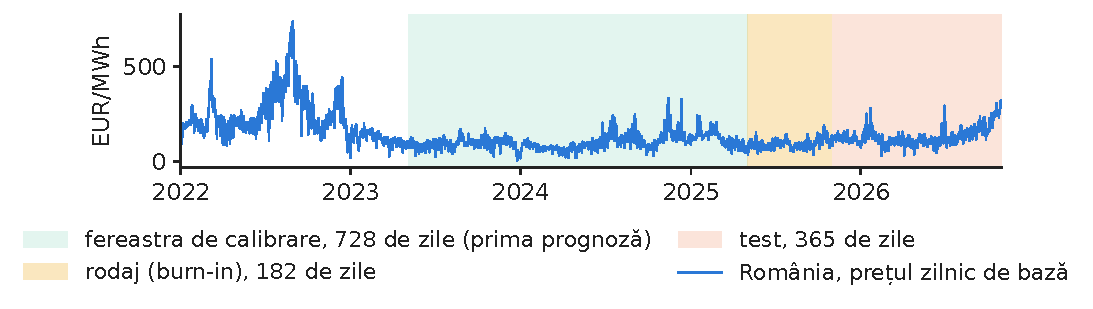
\includegraphics[width=\textwidth,height=0.398\textheight,keepaspectratio]{charts/ro/split_timeline.pdf}\end{center}\vspace{-3mm}
\chartsource{Sursa: energy-charts.info (Fraunhofer ISE); prețurile PZU ale OPCOM pentru România, prin ENTSO-E. Date: preț zilnic de bază, 2022-01-01 - 2026-10-31, zile de livrare CET.}
\vspace{0.5mm}
\begin{itemize}\setlength{\itemsep}{0pt}
  \item Calibrare = estimarea modelului, rodaj = prognoze folosite doar pentru intervale, test = măsurarea erorii.
  \item Reestimare zilnică pe fereastra care se încheie în ziua $d-1$, fără validare încrucișată aleatoare (K-fold).
\end{itemize}
\par\vfill\manager{cereți furnizorului de prognoze o testare retrospectivă (backtest) cu fereastră glisantă, nu ajustarea pe datele de estimare.}\par\vspace{0.5mm}
\par\vfill\noindent{\scriptsize\color{FooterGray}(Weron, 2014, IJF; Lago, Marcjasz, De Schutter \& Weron, 2021, APEN)}\hfill\qlink{EMQA\_L2\_split\_timeline}{Quantlets/L2/EMQA_L2_split_timeline}\par\vspace{0.5mm}
\end{frame}

\begin{frame}{Prețul mai vechi dă erori mai mari, cu excepția celui de acum o săptămînă}
\small
\begin{center}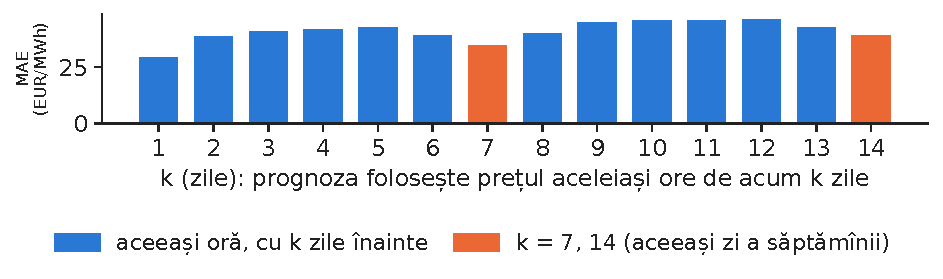
\includegraphics[width=\textwidth,height=0.409\textheight,keepaspectratio]{charts/ro/horizon_naive.pdf}\end{center}\vspace{-3mm}
\chartsource{Sursa: energy-charts.info (Fraunhofer ISE); prețurile PZU ale OPCOM pentru România, prin ENTSO-E. Date: anul de test 2025-11-01 - 2026-10-31, date orare.}
\vspace{0.5mm}
\begin{itemize}\setlength{\itemsep}{0pt}
  \item Cea mai simplă prognoză: $\hat P_{d,h}=P_{d-k,h}$, prețul aceleiași ore de acum $k$ zile
    \begin{itemize}\setlength{\itemsep}{0pt}
      \item MAE 29{,}37 EUR/MWh pentru $k=1$ (ieri), 38{,}52 pentru $k=2$, doar 34{,}41 pentru $k=7$ (aceeași zi a săptămînii)
    \end{itemize}
\end{itemize}
\par\vfill\manager{prognoza de la 12:00 din ziua $d-1$ privește următoarele 12--36 de ore
    \begin{itemize}\setlength{\itemsep}{0pt}
      \item Cel mai recent preț cunoscut este cel al zilei $d-1$.
    \end{itemize}}\par\vspace{0.5mm}
\par\vfill\noindent{\scriptsize\color{FooterGray}(calcule proprii, anul de test 1 noiembrie 2025 -- 31 octombrie 2026)}\hfill\qlink{EMQA\_L2\_horizon\_naive}{Quantlets/L2/EMQA_L2_horizon_naive}\par\vspace{0.5mm}
\end{frame}

\begin{frame}{Prognozele punctuale, probabilistice și de traiectorie răspund la întrebări diferite}
\footnotesize
\intuition{Prognoza punctuală dă un preț pentru fiecare oră, cea probabilistică dă distribuția prețului, iar cea de traiectorie dă scenarii pentru toate cele 24 de ore.}
\begin{columns}[T,onlytextwidth]
\begin{column}{0.54\textwidth}
\[ \underbrace{\hat P_{d,h}}_{\text{punctuală}}\quad\underbrace{\hat q^{\tau}_{d,h}:\ \Pr(P_{d,h}\le \hat q^{\tau}_{d,h})=\tau}_{\text{cuantilă}}\quad \underbrace{\{\hat P^{(s)}_{d,0},\dots,\hat P^{(s)}_{d,23}\}_{s=1}^{S}}_{\text{traiectorii}} \]{\footnotesize\begin{itemize}\setlength{\itemsep}{0pt}
  \item \textbf{\txtwhere}
    \begin{itemize}\setlength{\itemsep}{0pt}
      \item $d$ = ziua livrării
      \item $h$ = ora (CET)
      \item $\hat q^{\tau}_{d,h}$ = cuantila de nivel $\tau\in(0,1)$
      \item $s$ = scenariul
      \item $S$ = numărul de scenarii.
    \end{itemize}
\end{itemize}\par}
\end{column}
\begin{column}{0.43\textwidth}
\begin{itemize}\setlength{\itemsep}{1pt}
  \item \textbf{Pe datele din România}
    \begin{itemize}\setlength{\itemsep}{0pt}
      \item Corelația erorilor de prognoză între orele 12 și 13: 0{,}96
      \item Între orele 3 și 19: doar 0{,}13
    \end{itemize}
  \item \textbf{Cine folosește fiecare tip}
    \begin{itemize}\setlength{\itemsep}{0pt}
      \item Furnizorul de energie care cumpără un bloc de ore: prognoza punctuală
      \item Managerul de risc: cuantilele (cursul 4)
      \item Operatorul unei baterii: traiectoriile, deoarece cumpără energie într-o oră și o vinde în alta
    \end{itemize}
\end{itemize}
\end{column}
\end{columns}
\par\vfill\manager{înainte de a cumpăra o prognoză, stabiliți de care dintre cele trei tipuri are nevoie decizia dumneavoastră.}\par\vspace{0.5mm}
\par\vfill\noindent{\scriptsize\color{FooterGray}(Nowotarski \& Weron, 2018, RSER)}\hfill\tryit{notebook-ul Jupyter, secțiunea 7}\par\vspace{0.5mm}
\end{frame}

\subsection{Modele naive de referință și măsuri ale erorii}

\begin{frame}{Modelul naiv: prețul de ieri sau, lunea și în weekend, prețul de acum 7 zile}
\footnotesize
\intuition{Orice model trebuie să fie mai precis decît regula simplă pe care un trader ar aplica-o fără niciun model.}
\begin{columns}[T,onlytextwidth]
\begin{column}{0.52\textwidth}
\[ \hat P^{\text{naive}}_{d,h}=\begin{cases}P_{d-7,h}, & \text{lun., sîm., dum.}\\ P_{d-1,h}, & \text{mar.--vin.}\end{cases} \]\vspace{-2mm}\[ \hat P^{(7)}_{d,h}=P_{d-7,h} \]{\footnotesize\begin{itemize}\setlength{\itemsep}{0pt}
  \item \textbf{\txtwhere}
    \begin{itemize}\setlength{\itemsep}{0pt}
      \item $P_{d,h}$ = prețul zilei $d$, ora $h$ (EUR/MWh)
      \item $\hat P^{(7)}$ = modelul naiv sezonier: aceeași oră, cu o săptămînă în urmă.
    \end{itemize}
\end{itemize}\par}
\end{column}
\begin{column}{0.45\textwidth}
\begin{itemize}\setlength{\itemsep}{1pt}
  \item \textbf{De ce se schimbă regula} (MAE, EUR/MWh)
    \begin{itemize}\setlength{\itemsep}{0pt}
      \item Luni, sîmbătă, duminică: $d-7$ dă 29{,}87, $d-1$ dă 33{,}48
      \item Marți--vineri: $d-1$ dă 26{,}27, $d-7$ dă 37{,}83
    \end{itemize}
  \item \textbf{Anul de test}
    \begin{itemize}\setlength{\itemsep}{0pt}
      \item MAE: modelul naiv 27{,}82, naiv sezonier 34{,}41 EUR/MWh
      \item Prețul mediu este 134{,}46 EUR/MWh, deci eroarea naivă reprezintă circa o cincime din preț
    \end{itemize}
\end{itemize}
\end{column}
\end{columns}
\par\vfill\manager{cereți oricărui furnizor de prognoze rMAE față de această regulă naivă, calculată pe orele care vă interesează.}\par\vspace{0.5mm}
\par\vfill\noindent{\scriptsize\color{FooterGray}(Nogales et al., 2002, IEEE TPWRS; Weron, 2014, IJF)}\hfill\tryit{notebook-ul Jupyter, secțiunea 2}\par\vspace{0.5mm}
\end{frame}

\begin{frame}{Patru măsuri ale erorii și rMAE, care compară modelul cu cel naiv}
\footnotesize
\intuition{Erorile absolute sînt în EUR/MWh, cele pătratice penalizează salturile, rMAE compară cu modelul naiv.}
\begin{columns}[T,onlytextwidth]
\begin{column}{0.49\textwidth}
\[ \text{MAE}=\tfrac1N\textstyle\sum|e_{d,h}|,\quad \text{RMSE}=\sqrt{\tfrac1N\textstyle\sum e_{d,h}^2} \]\[ \text{sMAPE}=\tfrac1N\textstyle\sum\frac{2|e_{d,h}|}{|P_{d,h}|+|\hat P_{d,h}|},\quad \text{rMAE}=\frac{\text{MAE}_{\text{model}}}{\text{MAE}_{\text{naive}}} \]{\footnotesize\begin{itemize}\setlength{\itemsep}{0pt}
  \item \textbf{\txtwhere}
    \begin{itemize}\setlength{\itemsep}{0pt}
      \item $e_{d,h}=P_{d,h}-\hat P_{d,h}$ = eroarea
      \item $N$ = numărul perechilor (zi, oră)
      \item Eroarea procentuală absolută medie simetrică (sMAPE) $\in[0,200\%]$
      \item Valoare rMAE $<1$ = mai precis decît modelul naiv.
    \end{itemize}
\end{itemize}\par}
\end{column}
\begin{column}{0.48\textwidth}
\begin{itemize}\setlength{\itemsep}{1pt}
  \item \textbf{Pe datele din România}, anul de test 1 noiembrie 2025 -- 31 octombrie 2026
    \begin{itemize}\setlength{\itemsep}{0pt}
      \item Modelul naiv: MAE 27{,}82, RMSE 44{,}54, sMAPE 34{,}5\%
      \item LEAR mediat pe ferestre de calibrare (AW-LEAR, secțiunea 3): MAE 22{,}53, RMSE 36{,}35, rMAE 0{,}810
      \item Cel mai bun, ansamblul de 4 modele: rMAE 0{,}795, adică o eroare cu 20{,}5\% mai mică decît a modelului naiv
    \end{itemize}
  \item MAE este minimă pentru prognoza mediană, RMSE pentru cea medie.
\end{itemize}
\end{column}
\end{columns}
\par\vfill\manager{raportați biroului de tranzacționare MAE în EUR/MWh, iar conducerii rMAE, calculate pe aceleași ore.}\par\vspace{0.5mm}
\par\vfill\noindent{\scriptsize\color{FooterGray}(Hyndman \& Koehler, 2006, IJF; Lago et al., 2021, APEN)}\hfill\tryit{notebook-ul Jupyter, secțiunea 2}\par\vspace{0.5mm}
\end{frame}

\begin{frame}{Erorile procentuale nu funcționează la prețuri apropiate de zero sau negative}
\small
\begin{center}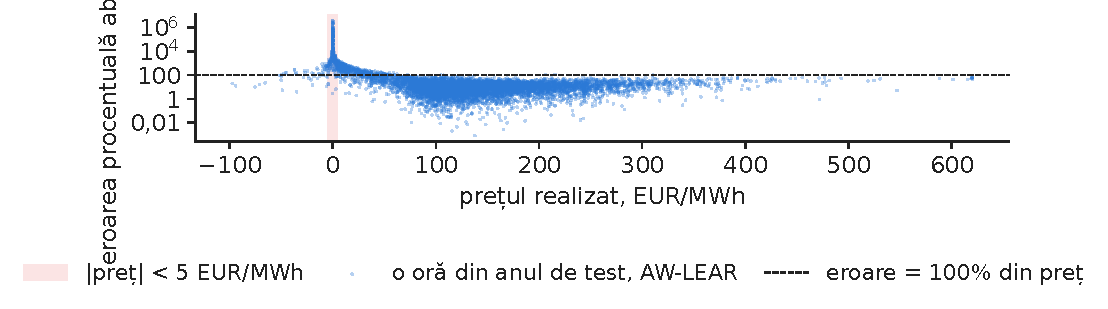
\includegraphics[width=\textwidth,height=0.355\textheight,keepaspectratio]{charts/ro/mape_fail.pdf}\end{center}\vspace{-3mm}
\chartsource{Sursa: energy-charts.info (Fraunhofer ISE); prețuri OPCOM; consum, producție eoliană și solară ENTSO-E (date Transelectrica pentru România). Date: anul de test 2025-11-01 - 2026-10-31, 8760 de ore.}
\vspace{0.5mm}
\begin{itemize}\setlength{\itemsep}{0pt}
  \item Eroarea procentuală absolută medie (MAPE) $=\tfrac1N\sum|e_{d,h}|/|P_{d,h}|$
    \begin{itemize}\setlength{\itemsep}{0pt}
      \item AW-LEAR: 5\,777{,}7\%, dar doar 32{,}4\% fără cele 387 de ore cu $|P|<5$ EUR/MWh.
    \end{itemize}
  \item Aceste puține ore generează 99{,}5\% din valoarea MAPE.
\end{itemize}
\par\vfill\manager{nu acceptați MAPE pentru prețurile energiei electrice
    \begin{itemize}\setlength{\itemsep}{0pt}
      \item Cereți MAE și rMAE.
    \end{itemize}}\par\vspace{0.5mm}
\par\vfill\noindent{\scriptsize\color{FooterGray}(Hyndman \& Koehler, 2006, IJF; Weron, 2014, IJF)}\hfill\qlink{EMQA\_L2\_mape\_fail}{Quantlets/L2/EMQA_L2_mape_fail}\par\vspace{0.5mm}
\end{frame}

\subsection{Testarea acurateței prognozelor}

\begin{frame}{Testul Diebold--Mariano arată dacă un model este cu adevărat mai precis decît altul}
\footnotesize
\intuition{Comparăm, zi de zi, eroarea medie a două modele; dacă diferența medie este mare față de variabilitatea ei, avantajul unui model nu se datorează întîmplării.}
\begin{columns}[T,onlytextwidth]
\begin{column}{0.51\textwidth}
\[ \Delta_d=\underbrace{\tfrac1{24}\textstyle\sum_h|e^{A}_{d,h}|}_{\text{modelul A}}-\underbrace{\tfrac1{24}\textstyle\sum_h|e^{B}_{d,h}|}_{\text{modelul B}},\qquad \text{DM}=\frac{\bar\Delta}{\sqrt{\hat\sigma^2_{\Delta}/n}} \]{\footnotesize\begin{itemize}\setlength{\itemsep}{0pt}
  \item \textbf{\txtwhere}
    \begin{itemize}\setlength{\itemsep}{0pt}
      \item $\Delta_d$ = diferența de eroare din ziua $d$
      \item $n$ = numărul zilelor de test
      \item $\hat\sigma^2_{\Delta}$ = varianța Newey--West cu 7 decalaje
      \item Valoarea $p=1-\Phi(\text{DM})$ sub 0{,}05 = B este semnificativ mai precis decît A.
    \end{itemize}
\end{itemize}\par}
\end{column}
\begin{column}{0.46\textwidth}
\begin{itemize}\setlength{\itemsep}{1pt}
  \item \textbf{Pe datele din România}, 365 de zile de test
    \begin{itemize}\setlength{\itemsep}{0pt}
      \item Modelul naiv față de AW-LEAR: DM 7{,}32, $p$ $<$0{,}001
      \item ARX mediat pe ferestre (AW-ARX) față de AW-LEAR: DM \ensuremath{-}0{,}83, $p$ = 0{,}797, diferență nesemnificativă statistic
      \item AW-LEAR față de ansamblul de 4 modele: DM 2{,}21, $p$ = 0{,}014
    \end{itemize}
  \item Media pe zi elimină corelația dintre cele 24 de ore ale aceleiași zile (varianta multivariată a testului).
\end{itemize}
\end{column}
\end{columns}
\par\vfill\manager{schimbați modelul numai dacă îmbunătățirea este semnificativă pe orele care vă interesează.}\par\vspace{0.5mm}
\par\vfill\noindent{\scriptsize\color{FooterGray}(Diebold \& Mariano, 1995, JBES; Ziel \& Weron, 2018, ENEECO)}\hfill\tryit{notebook-ul Jupyter, secțiunea 2}\par\vspace{0.5mm}
\end{frame}

\begin{frame}{Matricea testelor DM: care modele sînt semnificativ mai precise în România}
\small
\begin{center}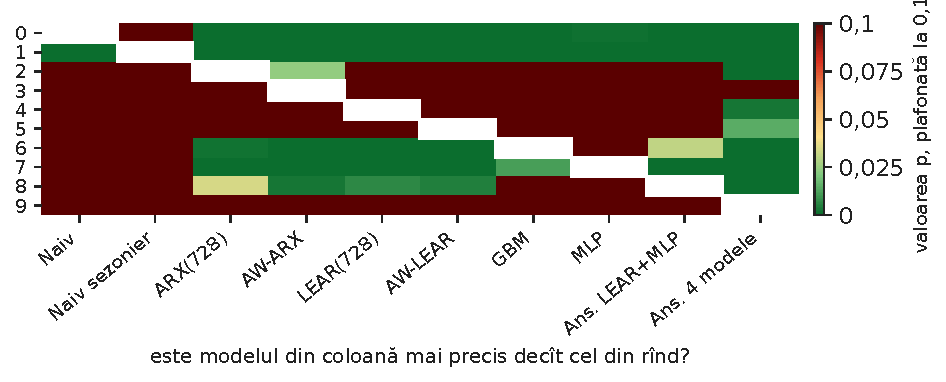
\includegraphics[width=\textwidth,height=0.466\textheight,keepaspectratio]{charts/ro/dm_matrix.pdf}\end{center}\vspace{-3mm}
\chartsource{Sursa: energy-charts.info (Fraunhofer ISE); prețuri OPCOM; producție și fluxuri ENTSO-E (date Transelectrica pentru România); Yahoo Finance (SparkChange EUA ETC). Date: anul de test 2025-11-01 - 2026-10-31, 365 de zile; valori p unilaterale.}
\vspace{0.5mm}
\begin{itemize}\setlength{\itemsep}{0pt}
  \item 8 dintre celelalte 9 modele sînt semnificativ mai precise decît modelul naiv, la pragul de 5\%
    \begin{itemize}\setlength{\itemsep}{0pt}
      \item O celulă verde = modelul din coloană este semnificativ mai precis decît cel din rînd.
    \end{itemize}
\end{itemize}
\par\vfill\manager{citiți fiecare coloană de sus în jos
    \begin{itemize}\setlength{\itemsep}{0pt}
      \item Multe celule verzi indică un model pentru care merită să plătiți.
    \end{itemize}}\par\vspace{0.5mm}
\par\vfill\noindent{\scriptsize\color{FooterGray}(Ziel \& Weron, 2018, ENEECO; Lago et al., 2021, APEN)}\hfill\qlink{EMQA\_L2\_dm\_matrix}{Quantlets/L2/EMQA_L2_dm_matrix}\par\vspace{0.5mm}
\end{frame}


\section{Modele expert: ARX și LEAR}

\subsection{Modelul expert ARX}

\begin{frame}{Modelul expert ARX: prețuri recente, calendar și variabile fundamentale}
\footnotesize
\intuition{O regresie liniară pentru fiecare oră, cu variabilele urmărite de un trader.}
\begin{columns}[T,onlytextwidth]
\begin{column}{0.55\textwidth}
\[ \begin{aligned} Y_{d,h}=\beta_0&+\underbrace{\beta_1Y_{d-1,h}+\beta_2Y_{d-2,h}+\beta_3Y_{d-7,h}}_{\text{autoregresie}}\\&+\underbrace{\beta_4Y_{d-1,23}+\beta_5Y^{\min}_{d-1}+\beta_6Y^{\max}_{d-1}}_{\text{forma zilei precedente}}\\&+\underbrace{\beta_7\tilde L_{d,h}+\beta_8\tilde R_{d,h}}_{\text{fundamentale din } d-2}+\underbrace{\textstyle\sum_{j}\delta_jD^{j}_d}_{\text{lun., sîm., dum.}}+\varepsilon_{d,h} \end{aligned} \]{\footnotesize\begin{itemize}\setlength{\itemsep}{0pt}
  \item \textbf{\txtwhere}
    \begin{itemize}\setlength{\itemsep}{0pt}
      \item $Y$ = prețul transformat asinh
      \item $\tilde L_{d,h}=L_{d-2,h}$ = consumul, $\tilde R_{d,h}$ = producția eoliană și solară din $d-2$, standardizate.
    \end{itemize}
\end{itemize}\par}
\end{column}
\begin{column}{0.42\textwidth}
\begin{itemize}\setlength{\itemsep}{1pt}
  \item \textbf{Estimare}
    \begin{itemize}\setlength{\itemsep}{0pt}
      \item Metoda celor mai mici pătrate (OLS), separat pentru fiecare $h$
      \item 12 regresori pentru fiecare oră, ca în tema 1
    \end{itemize}
  \item \textbf{Pe datele din România}, ARX(728)
    \begin{itemize}\setlength{\itemsep}{0pt}
      \item Reestimat zilnic pe ultimele 728 de zile
      \item MAE 22{,}72 EUR/MWh, rMAE 0{,}817
    \end{itemize}
\end{itemize}
\end{column}
\end{columns}
\par\vfill\manager{acesta este modelul de depășit înainte să cumpărați o rețea neuronală.}\par\vspace{0.5mm}
\par\vfill\noindent{\scriptsize\color{FooterGray}(Ziel \& Weron, 2018, ENEECO; Weron, 2014, IJF)}\hfill\tryit{notebook-ul Jupyter, secțiunea 3}\par\vspace{0.5mm}
\end{frame}

\begin{frame}{Coeficienții modelului ARX diferă de la o oră la alta}
\small
\begin{center}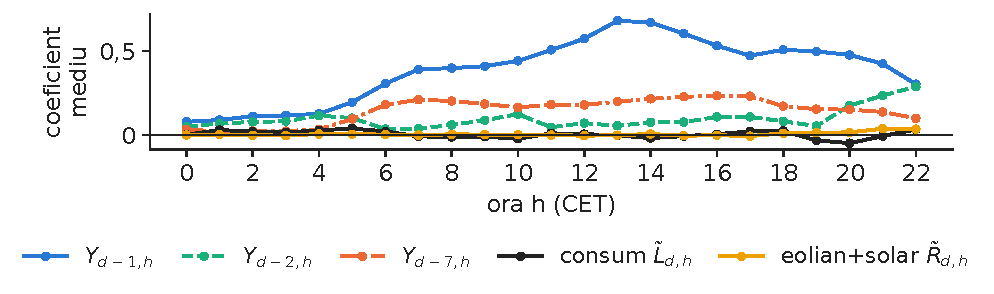
\includegraphics[width=\textwidth,height=0.455\textheight,keepaspectratio]{charts/ro/arx_coef.pdf}\end{center}\vspace{-3mm}
\chartsource{Sursa: energy-charts.info (Fraunhofer ISE); prețuri OPCOM; consum, producție eoliană și solară ENTSO-E (date Transelectrica pentru România). Date: ARX(728), media celor 365 de estimări zilnice din anul de test.}
\vspace{0.5mm}
\begin{itemize}\setlength{\itemsep}{0pt}
  \item $Y_{d-1,h}$ (aceeași oră, ieri) are coeficientul maxim la ora 13 (0{,}68) și minim la ora 0 (0{,}08)
    \begin{itemize}\setlength{\itemsep}{0pt}
      \item Noaptea contează mai mult ultima oră a zilei $d-1$ (pînă la 0{,}73).
    \end{itemize}
  \item Consumul și producția eoliană și solară au coeficienți apropiați de zero: datele din $d-2$ adaugă puțin.
\end{itemize}
\par\vfill\manager{cîte un model pe oră permite ca vîrful de seară să depindă de alți factori decît noaptea.}\par\vspace{0.5mm}
\par\vfill\noindent{\scriptsize\color{FooterGray}(estimare proprie, ARX(728))}\hfill\qlink{EMQA\_L2\_arx\_coef}{Quantlets/L2/EMQA_L2_arx_coef}\par\vspace{0.5mm}
\end{frame}

\begin{frame}{Variabilele fundamentale din ziua $d-2$ aproape că nu îmbunătățesc prognoza}
\footnotesize
\begin{columns}[T,onlytextwidth]
\begin{column}{0.50\textwidth}
{\footnotesize\renewcommand{\arraystretch}{1.25}\setlength{\tabcolsep}{4pt}
\begin{tabular}{@{}p{0.52\linewidth}rrr@{}}\toprule
ARX(728), anul de test & MAE & RMSE & rMAE \\ \midrule
numai prețuri și calendar & 22{,}63 & 36{,}49 & 0{,}813 \\
+ consum, producție eoliană și solară din $d-2$ & 22{,}72 & 36{,}62 & 0{,}817 \\
+ hidro, nuclear, import net, EUA din $d-2$ & 22{,}72 & 36{,}50 & 0{,}817 \\
\bottomrule\end{tabular}}
\par\vspace{0.5mm}{\scriptsize \begin{itemize}\setlength{\itemsep}{0pt}
  \item Valorile lipsă ale variabilelor fundamentale se înlocuiesc cu ultima valoare observată (pentru nuclear, în 29 de zile).
  \item EUA = prețul de închidere al titlului SparkChange din ziua $d-2$, folosit ca aproximare a prețului certificatului de emisii.
\end{itemize}}
\end{column}
\begin{column}{0.47\textwidth}
\begin{itemize}\setlength{\itemsep}{1pt}
  \item \textbf{De ce atît de puțin}
    \begin{itemize}\setlength{\itemsep}{0pt}
      \item Informația din ziua $d-2$ este deja inclusă în prețul zilei $d-1$
      \item De exemplu, opririle centralei nucleare de la Cernavodă intră în model cu două zile întîrziere
    \end{itemize}
  \item \textbf{Ce ar ajuta}
    \begin{itemize}\setlength{\itemsep}{0pt}
      \item Prognozele de consum și de producție eoliană și solară pentru ziua $d$ (ENTSO-E, Transelectrica)
      \item Sînt publicate înainte de 12:00 în ziua $d-1$, deci pot fi folosite, dar nu fac parte din datele noastre gratuite
    \end{itemize}
\end{itemize}
\end{column}
\end{columns}
\par\vfill\manager{cumpărați prognozele TSO de consum și de producție regenerabilă pentru ziua următoare înainte de a plăti pentru un model mai complex.}\par\vspace{0.5mm}
\par\vfill\noindent{\scriptsize\color{FooterGray}(estimare proprie; Lago et al., 2021, APEN)}\hfill\tryit{notebook-ul Jupyter, secțiunea 3}\par\vspace{0.5mm}
\end{frame}

\begin{frame}{Cîte un model pentru fiecare oră este mai precis decît un model comun}
\small
\begin{center}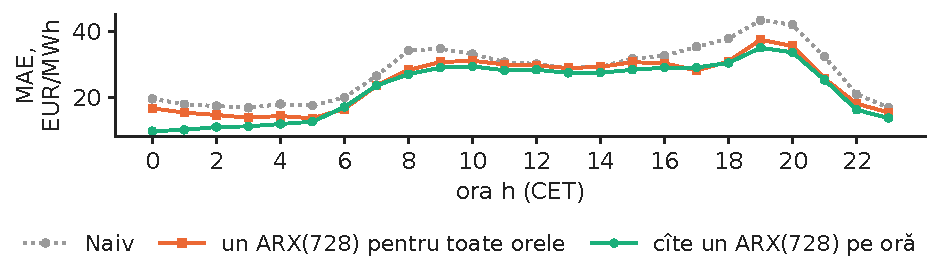
\includegraphics[width=\textwidth,height=0.426\textheight,keepaspectratio]{charts/ro/per_hour_single.pdf}\end{center}\vspace{-3mm}
\chartsource{Sursa: energy-charts.info (Fraunhofer ISE); prețuri OPCOM; consum, producție eoliană și solară ENTSO-E (date Transelectrica pentru România). Date: anul de test 2025-11-01 - 2026-10-31.}
\vspace{0.5mm}
\begin{itemize}\setlength{\itemsep}{0pt}
  \item MAE: 22{,}72 cu cîte un model pe oră, 24{,}54 EUR/MWh cu un model comun (constantă proprie fiecărei ore, pante comune)
    \begin{itemize}\setlength{\itemsep}{0pt}
      \item Modelul comun este mai slab în 21 din 24 de ore.
    \end{itemize}
\end{itemize}
\par\vfill\manager{din 1 octombrie 2025 se tranzacționează sferturi de oră, deci aceeași alegere apare pentru cele 96 de intervale ale zilei.}\par\vspace{0.5mm}
\par\vfill\noindent{\scriptsize\color{FooterGray}(Ziel \& Weron, 2018, ENEECO)}\hfill\qlink{EMQA\_L2\_per\_hour\_single}{Quantlets/L2/EMQA_L2_per_hour_single}\par\vspace{0.5mm}
\end{frame}

\subsection{Transformări de stabilizare a varianței}

\begin{frame}{Transformarea asinh atenuează salturile și acceptă prețuri negative}
\small
\begin{center}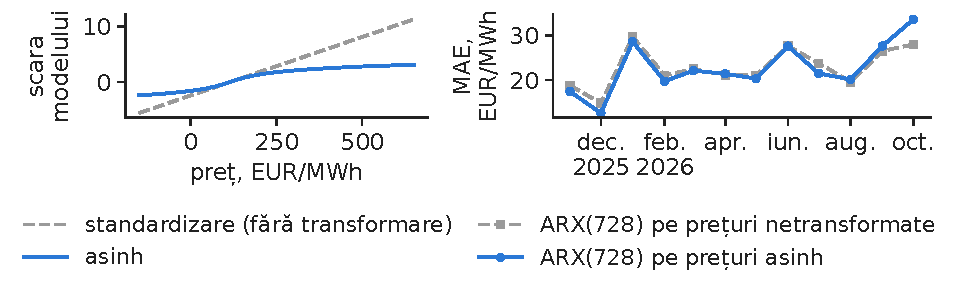
\includegraphics[width=\textwidth,height=0.431\textheight,keepaspectratio]{charts/ro/vst.pdf}\end{center}\vspace{-3mm}
\chartsource{Sursa: energy-charts.info (Fraunhofer ISE); prețuri OPCOM; consum, producție eoliană și solară ENTSO-E (date Transelectrica pentru România). Date: stînga, mediana și scala din ultima fereastră; dreapta, anul de test 2025-11-01 - 2026-10-31.}
\vspace{0.5mm}
\begin{itemize}\setlength{\itemsep}{0pt}
  \item Transformarea de stabilizare a varianței (VST): $Y=\asinh((P-m)/s)$
    \begin{itemize}\setlength{\itemsep}{0pt}
      \item $m$ = mediana, $s$ = 1{,}4826 $\times$ abaterea absolută mediană (MAD), ambele din fereastra de calibrare.
    \end{itemize}
  \item MAE pentru ARX(728): 22{,}86 pe prețuri netransformate, 22{,}72 cu asinh
    \begin{itemize}\setlength{\itemsep}{0pt}
      \item Pentru RMSE ordinea se inversează (35{,}85 față de 36{,}62).
    \end{itemize}
\end{itemize}
\par\vfill\manager{funcția asinh este definită și pentru valori negative, unde logaritmul nu poate fi folosit.}\par\vspace{0.5mm}
\par\vfill\noindent{\scriptsize\color{FooterGray}(Uniejewski, Weron \& Ziel, 2018, IEEE TPWRS)}\hfill\qlink{EMQA\_L2\_vst}{Quantlets/L2/EMQA_L2_vst}\par\vspace{0.5mm}
\end{frame}

\subsection{Autoregresia estimată cu LASSO}

\begin{frame}{LEAR pornește de la 247 de regresori, iar LASSO îi elimină pe cei mai mulți}
\footnotesize
\intuition{O penalizare a mărimii coeficienților îi face zero pe cei inutili, deci datele aleg regresorii.}
\begin{columns}[T,onlytextwidth]
\begin{column}{0.53\textwidth}
\[ \hat{\bm\beta}_h=\arg\min_{\bm\beta}\Big\{\underbrace{\textstyle\sum_{d\in\text{cal}}(Y_{d,h}-\mathbf x_d^{\top}\bm\beta)^2}_{\text{ajustare}}+\underbrace{\lambda_h\textstyle\sum_j|\beta_j|}_{\text{penalizare}}\Big\} \]{\footnotesize\begin{itemize}\setlength{\itemsep}{0pt}
  \item \textbf{\txtwhere}
    \begin{itemize}\setlength{\itemsep}{0pt}
      \item $\mathbf x_d$ = 247 de regresori: cele 24 de prețuri din $d-1,d-2,d-3,d-7$ (96), consumul și producția eoliană și solară din $d-2,d-3,d-7$ (144), 7 indicatori ai zilei
      \item $\lambda_h$ = intensitatea penalizării, aleasă zilnic prin criteriul informațional Akaike (AIC).
    \end{itemize}
\end{itemize}\par}
\end{column}
\begin{column}{0.44\textwidth}
\begin{itemize}\setlength{\itemsep}{1pt}
  \item \textbf{Pe datele din România}, LEAR(728)
    \begin{itemize}\setlength{\itemsep}{0pt}
      \item Rămîn în medie 42 din 247 (17\%), între 8 și 121
      \item MAE 22{,}62; media prognozelor estimate pe 364, 546 și 728 de zile (AW-LEAR): 22{,}53 EUR/MWh
    \end{itemize}
  \item \textbf{Cum se alege corect $\lambda$}
    \begin{itemize}\setlength{\itemsep}{0pt}
      \item Printr-un criteriu informațional sau pe un bloc de validare care se încheie înaintea zilei prognozate
      \item Niciodată pe anul de test
    \end{itemize}
\end{itemize}
\end{column}
\end{columns}
\par\vfill\manager{un model LASSO este ușor de interpretat: regresorii păstrați arată ce influențează prețul în fiecare oră.}\par\vspace{0.5mm}
\par\vfill\noindent{\scriptsize\color{FooterGray}(Tibshirani, 1996; Uniejewski, Nowotarski \& Weron, 2016; Lago et al., 2021)}\hfill\tryit{notebook-ul Jupyter, secțiunea 4}\par\vspace{0.5mm}
\end{frame}

\begin{frame}{LEAR păstrează prețul aceleiași ore de ieri și ziua săptămînii}
\small
\begin{center}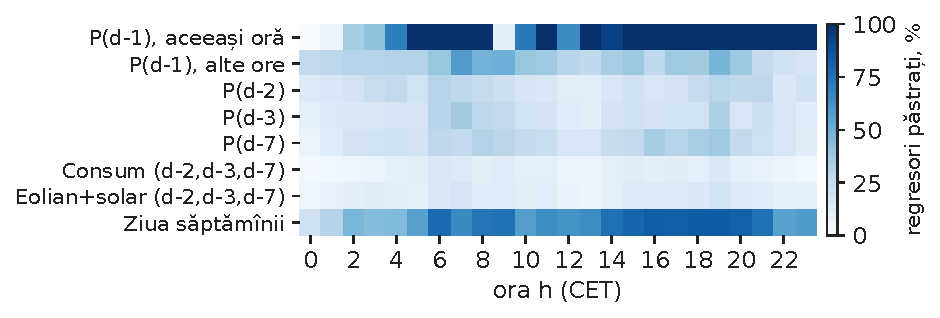
\includegraphics[width=\textwidth,height=0.499\textheight,keepaspectratio]{charts/ro/lear_sel.pdf}\end{center}\vspace{-3mm}
\chartsource{Sursa: energy-charts.info (Fraunhofer ISE); prețuri OPCOM; consum, producție eoliană și solară ENTSO-E (date Transelectrica pentru România). Date: LEAR(728), 365 de estimări zilnice din anul de test.}
\vspace{0.5mm}
\begin{itemize}\setlength{\itemsep}{0pt}
  \item Procentul mediu al regresorilor păstrați din fiecare grupă: $P_{d-1,h}$ (aceeași oră, ieri) 79\%, ziua săptămînii 64\%, consum 9\%, producție eoliană și solară 11\%.
\end{itemize}
\par\vfill\manager{pentru cîștiguri reale aveți nevoie de prognoze ale variabilelor fundamentale pentru ziua $d$.}\par\vspace{0.5mm}
\par\vfill\noindent{\scriptsize\color{FooterGray}(estimare proprie, LEAR(728), anul de test 1 noiembrie 2025 -- 31 octombrie 2026)}\hfill\qlink{EMQA\_L2\_lear\_sel}{Quantlets/L2/EMQA_L2_lear_sel}\par\vspace{0.5mm}
\end{frame}


\section{Ferestre, combinații și învățare automată}

\subsection{Ferestre de calibrare}

\begin{frame}{Ferestrele scurte se adaptează, cele lungi sînt stabile: mediați prognozele}
\footnotesize
\intuition{În loc să ghiciți lungimea optimă a ferestrei de calibrare, estimați modelul pe mai multe ferestre și faceți media prognozelor.}
\begin{columns}[T,onlytextwidth]
\begin{column}{0.52\textwidth}
\[ \hat P^{\text{AW}}_{d,h}=\frac1{|\mathcal T|}\sum_{T\in\mathcal T}\underbrace{\hat P^{(T)}_{d,h}}_{\text{fereastră de } T \text{ zile}} \]{\footnotesize\begin{itemize}\setlength{\itemsep}{0pt}
  \item \textbf{\txtwhere}
    \begin{itemize}\setlength{\itemsep}{0pt}
      \item $\hat P^{(T)}_{d,h}$ = prognoza estimată pe ultimele $T$ zile (fereastră glisantă)
      \item ARX: $\mathcal T=\{56,84,112,714,721,728\}$
      \item LEAR: $\mathcal T=\{364,546,728\}$
      \item Medierea pe ferestre de calibrare (AW).
    \end{itemize}
\end{itemize}\par}
\end{column}
\begin{column}{0.45\textwidth}
\begin{itemize}\setlength{\itemsep}{1pt}
  \item \textbf{Pe datele din România}, MAE în EUR/MWh
    \begin{itemize}\setlength{\itemsep}{0pt}
      \item ARX(56) 24{,}44, ARX(112) 23{,}41, ARX(728) 22{,}72
      \item AW-ARX 22{,}30, mai precis decît modelul estimat pe oricare fereastră
      \item LEAR(364) 22{,}96, LEAR(728) 22{,}62, AW-LEAR 22{,}53
    \end{itemize}
  \item Combinarea ferestrelor scurte (56--112 zile) cu cele lungi (714--728 de zile) aduce atît adaptare, cît și stabilitate.
\end{itemize}
\end{column}
\end{columns}
\par\vfill\manager{cînd piața își schimbă regimul (2022, 2024), ferestrele scurte reacționează primele
    \begin{itemize}\setlength{\itemsep}{0pt}
      \item Păstrați-le în medie.
    \end{itemize}}\par\vspace{0.5mm}
\par\vfill\noindent{\scriptsize\color{FooterGray}(Hubicka, Marcjasz \& Weron, 2019; Marcjasz, Serafin \& Weron, 2018)}\hfill\tryit{notebook-ul Jupyter, secțiunea 5}\par\vspace{0.5mm}
\end{frame}

\begin{frame}{Media pe ferestre este mai precisă decît cea mai bună fereastră}
\small
\begin{center}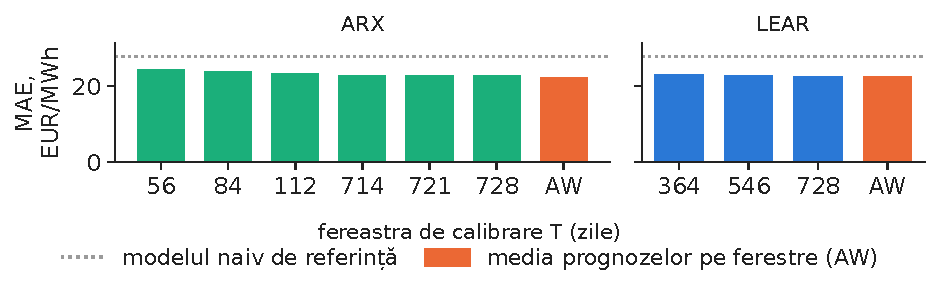
\includegraphics[width=\textwidth,height=0.459\textheight,keepaspectratio]{charts/ro/windows.pdf}\end{center}\vspace{-3mm}
\chartsource{Sursa: energy-charts.info (Fraunhofer ISE); prețuri OPCOM; consum, producție eoliană și solară ENTSO-E (date Transelectrica pentru România). Date: anul de test 2025-11-01 - 2026-10-31.}
\vspace{0.5mm}
\begin{itemize}\setlength{\itemsep}{0pt}
  \item MAE: AW-ARX 22{,}30, față de 22{,}68 pentru cea mai bună fereastră, ARX(714)
    \begin{itemize}\setlength{\itemsep}{0pt}
      \item Linia punctată = modelul naiv, 27{,}82 EUR/MWh.
    \end{itemize}
\end{itemize}
\par\vfill\manager{nu trebuie să știți dinainte care fereastră este potrivită
    \begin{itemize}\setlength{\itemsep}{0pt}
      \item Faceți media prognozelor obținute pe o fereastră scurtă și pe una lungă.
    \end{itemize}}\par\vspace{0.5mm}
\par\vfill\noindent{\scriptsize\color{FooterGray}(Hubicka, Marcjasz \& Weron, 2019, IEEE TSTE)}\hfill\qlink{EMQA\_L2\_windows}{Quantlets/L2/EMQA_L2_windows}\par\vspace{0.5mm}
\end{frame}

\subsection{Combinarea prognozelor}

\begin{frame}{Combinarea modelelor: erorile care nu coincid se compensează}
\footnotesize
\intuition{Dacă două modele greșesc în zile diferite, media simplă a prognozelor lor greșește mai rar decît fiecare dintre ele.}
\begin{columns}[T,onlytextwidth]
\begin{column}{0.48\textwidth}
\[ \hat P^{\text{ens}}_{d,h}=\frac1K\sum_{k=1}^{K}\hat P^{(k)}_{d,h},\quad \Var(\bar e)=\frac{\bar\sigma^2}{K}\big(1+(K-1)\bar\rho\big) \]{\footnotesize\begin{itemize}\setlength{\itemsep}{0pt}
  \item \textbf{\txtwhere}
    \begin{itemize}\setlength{\itemsep}{0pt}
      \item $K$ = numărul de modele
      \item $\bar\sigma^2$ = varianța medie a erorilor
      \item $\bar\rho$ = corelația medie a erorilor
      \item Cu cît $\bar\rho$ e mai mic, cu atît cîștigul e mai mare
      \item Ponderile egale nu se estimează.
    \end{itemize}
\end{itemize}\par}
\end{column}
\begin{column}{0.49\textwidth}
\begin{itemize}\setlength{\itemsep}{1pt}
  \item \textbf{Pe datele din România}, ansamblul de 4 modele
    \begin{itemize}\setlength{\itemsep}{0pt}
      \item AW-ARX, AW-LEAR, un model gradient boosting (GBM) și un perceptron multistrat (MLP), ponderi egale
      \item MAE 22{,}13 EUR/MWh, rMAE 0{,}795, cel mai bun dintre toate modelele
      \item Mai bun decît AW-LEAR în 8 din 12 luni și în 15 din 24 de ore
      \item Testul DM față de AW-LEAR: $p$ = 0{,}014
    \end{itemize}
  \item Cei doi membri mai slabi (GBM, MLP) ajută totuși, deoarece erorile lor diferă.
\end{itemize}
\end{column}
\end{columns}
\par\vfill\manager{cereți furnizorilor de prognoze serii pe care să le puteți combina cu ale dumneavoastră, nu un singur model „cel mai bun”.}\par\vspace{0.5mm}
\par\vfill\noindent{\scriptsize\color{FooterGray}(Bates \& Granger, 1969; Nowotarski \& Weron, 2015)}\hfill\tryit{notebook-ul Jupyter, secțiunea 5}\par\vspace{0.5mm}
\end{frame}

\begin{frame}{Clasamentul modelelor pe anul de test în România}
\small
\begin{center}{\scriptsize\renewcommand{\arraystretch}{1.02}\setlength{\tabcolsep}{4pt}
\begin{tabular}{@{}lrrrr@{}}\toprule
Model & MAE & RMSE & sMAPE, \% & rMAE \\ \midrule
Naiv & \cellcolor{Forest!4}27{,}82 & \cellcolor{Forest!6}44{,}54 & \cellcolor{Crimson!10}34{,}5 & \cellcolor{Forest!4}1{,}000 \\
Naiv sezonier & \cellcolor{Crimson!55}34{,}41 & \cellcolor{Crimson!55}55{,}48 & \cellcolor{Crimson!55}39{,}4 & \cellcolor{Crimson!55}1{,}237 \\
ARX(56) & \cellcolor{Forest!34}24{,}44 & \cellcolor{Forest!31}40{,}09 & \cellcolor{Forest!31}30{,}0 & \cellcolor{Forest!34}0{,}879 \\
ARX(728) & \cellcolor{Forest!50}22{,}72 & \cellcolor{Forest!50}36{,}62 & \cellcolor{Forest!51}27{,}8 & \cellcolor{Forest!50}0{,}817 \\
AW-ARX & \cellcolor{Forest!53}22{,}30 & \cellcolor{Forest!52}36{,}34 & \cellcolor{Forest!54}27{,}6 & \cellcolor{Forest!53}0{,}802 \\
ARX(728), model comun & \cellcolor{Forest!33}24{,}54 & \cellcolor{Forest!43}37{,}97 & \cellcolor{Forest!36}29{,}5 & \cellcolor{Forest!33}0{,}882 \\
ARX(728), fără VST & \cellcolor{Forest!48}22{,}86 & \cellcolor{Forest!54}35{,}85 & \cellcolor{Forest!46}28{,}4 & \cellcolor{Forest!48}0{,}822 \\
LEAR(364) & \cellcolor{Forest!48}22{,}96 & \cellcolor{Forest!49}36{,}80 & \cellcolor{Forest!49}28{,}1 & \cellcolor{Forest!48}0{,}825 \\
LEAR(728) & \cellcolor{Forest!51}22{,}62 & \cellcolor{Forest!52}36{,}36 & \cellcolor{Forest!53}27{,}7 & \cellcolor{Forest!51}0{,}813 \\
AW-LEAR & \cellcolor{Forest!51}22{,}53 & \cellcolor{Forest!52}36{,}35 & \cellcolor{Forest!53}27{,}7 & \cellcolor{Forest!51}0{,}810 \\
GBM & \cellcolor{Forest!38}24{,}05 & \cellcolor{Forest!44}37{,}73 & \cellcolor{Forest!44}28{,}7 & \cellcolor{Forest!38}0{,}864 \\
MLP & \cellcolor{Forest!24}25{,}54 & \cellcolor{Forest!31}40{,}05 & \cellcolor{Forest!33}29{,}8 & \cellcolor{Forest!24}0{,}918 \\
Ansamblu LEAR+MLP & \cellcolor{Forest!46}23{,}12 & \cellcolor{Forest!48}36{,}95 & \cellcolor{Forest!49}28{,}1 & \cellcolor{Forest!46}0{,}831 \\
Ansamblu de 4 modele & \cellcolor{Forest!55}22{,}13 & \cellcolor{Forest!55}35{,}76 & \cellcolor{Forest!55}27{,}4 & \cellcolor{Forest!55}0{,}795 \\
\bottomrule\end{tabular}}\end{center}\vspace{-2mm}
\par\vspace{0.5mm}{\scriptsize \begin{itemize}\setlength{\itemsep}{0pt}
  \item Anul de test 1 noiembrie 2025 -- 31 octombrie 2026, 8\,760 de ore; verde = mai precis, roșu = mai puțin precis, separat pe fiecare coloană.
  \item Fără cele 2 zile cu schimbarea orei, MAE pentru AW-LEAR este 22{,}48; clasamentul nu se schimbă.
\end{itemize}}
\par\vfill\noindent{\scriptsize\color{FooterGray}(Weron, 2014, IJF; Lago, Marcjasz, De Schutter \& Weron, 2021, APEN)}\hfill\tryit{notebook-ul Jupyter, secțiunea 5}\par\vspace{0.5mm}
\end{frame}

\subsection{Învățarea automată: introducere la cursul 7}

\begin{frame}{Gradient boosting: mulți arbori mici, fiecare corectîndu-i pe cei anteriori}
\footnotesize
\intuition{Arborii surprind praguri și interacțiuni (de exemplu, vînt slab și consum mare seara), pe care un model liniar nu le vede.}
\begin{columns}[T,onlytextwidth]
\begin{column}{0.50\textwidth}
\[ F_m(\mathbf x)=F_{m-1}(\mathbf x)+\nu\,f_m(\mathbf x) \]\vspace{-2mm}\[ f_m=\arg\min_f\textstyle\sum_i\big(r_i^{(m)}-f(\mathbf x_i)\big)^2 \]{\footnotesize\begin{itemize}\setlength{\itemsep}{0pt}
  \item \textbf{\txtwhere}
    \begin{itemize}\setlength{\itemsep}{0pt}
      \item $f_m$ = un arbore de regresie mic
      \item $r_i^{(m)}=Y_i-F_{m-1}(\mathbf x_i)$ = reziduul curent
      \item $\nu=0{,}05$ = rata de învățare
      \item 500 de arbori.
    \end{itemize}
\end{itemize}\par}
\end{column}
\begin{column}{0.47\textwidth}
\begin{itemize}\setlength{\itemsep}{1pt}
  \item \textbf{Modelul nostru de gradient boosting (GBM)}
    \begin{itemize}\setlength{\itemsep}{0pt}
      \item Un singur model pentru toate orele, ora fiind o variabilă; 20 de variabile, toate cunoscute la 12:00 în ziua $d-1$
      \item Reestimat la începutul fiecărei luni de test (12 reestimări), pe toate zilele anterioare
    \end{itemize}
  \item \textbf{Rezultat}
    \begin{itemize}\setlength{\itemsep}{0pt}
      \item MAE 24{,}05, rMAE 0{,}864; pe ansamblul anului, mai puțin precis decît AW-LEAR
      \item Dar cel mai bun model individual în săptămîna de criză (MAE 34{,}35)
    \end{itemize}
\end{itemize}
\end{column}
\end{columns}
\par\vfill\manager{arborii merită incluși într-un ansamblu, chiar dacă nu sînt cei mai buni luați separat.}\par\vspace{0.5mm}
\par\vfill\noindent{\scriptsize\color{FooterGray}(Friedman, 2001, Ann.\ Stat.; Lago et al., 2021, APEN)}\hfill\tryit{notebook-ul Jupyter, secțiunea 6}\par\vspace{0.5mm}
\end{frame}

\begin{frame}{Rețele neuronale: 24 de prețuri dintr-un singur vector de intrare}
\footnotesize
\intuition{O rețea cu 24 de ieșiri prognozează toată ziua deodată, ca rețeaua neuronală profundă (DNN) din Lago et al.}
\begin{columns}[T,onlytextwidth]
\begin{column}{0.50\textwidth}
\[ \hat{\mathbf Y}_d=W_3\,\phi\big(W_2\,\phi(W_1\mathbf x_d+b_1)+b_2\big)+b_3\in\mathbb R^{24} \]{\footnotesize\begin{itemize}\setlength{\itemsep}{0pt}
  \item \textbf{\txtwhere}
    \begin{itemize}\setlength{\itemsep}{0pt}
      \item $\mathbf x_d$ = cei 247 de regresori LEAR și 4 variabile fundamentale din $d-2$
      \item $\phi$ = unitatea liniară rectificată (ReLU)
      \item Straturi ascunse de 128 și 64 de neuroni
      \item Perceptron multistrat (MLP).
    \end{itemize}
\end{itemize}\par}
\end{column}
\begin{column}{0.47\textwidth}
\begin{itemize}\setlength{\itemsep}{1pt}
  \item \textbf{Disciplina seriilor de timp}
    \begin{itemize}\setlength{\itemsep}{0pt}
      \item Numărul de epoci, ales pe ultimele 15\% din zile (mediana: 20)
      \item Media a 4 inițializări; reestimare lunară; standardizare pe zilele de antrenare
    \end{itemize}
  \item \textbf{Rezultat}
    \begin{itemize}\setlength{\itemsep}{0pt}
      \item MAE 25{,}54, rMAE 0{,}918; o rețea mică, neoptimizată, nu depășește LEAR
      \item Rețeaua DNN optimizată de Lago et al.\ (2021) obține rezultate mai bune (cursul 7)
    \end{itemize}
\end{itemize}
\end{column}
\end{columns}
\par\vfill\manager{o rețea neuronală cere ani de date și o calibrare atentă
    \begin{itemize}\setlength{\itemsep}{0pt}
      \item Altfel, păstrați LEAR.
    \end{itemize}}\par\vspace{0.5mm}
\par\vfill\noindent{\scriptsize\color{FooterGray}(Lago, Marcjasz, De Schutter \& Weron, 2021, APEN)}\hfill\tryit{notebook-ul Jupyter, secțiunea 6}\par\vspace{0.5mm}
\end{frame}

\begin{frame}{Pe ore, învățarea automată ajută în cadrul ansamblului, nu luată separat}
\small
\begin{center}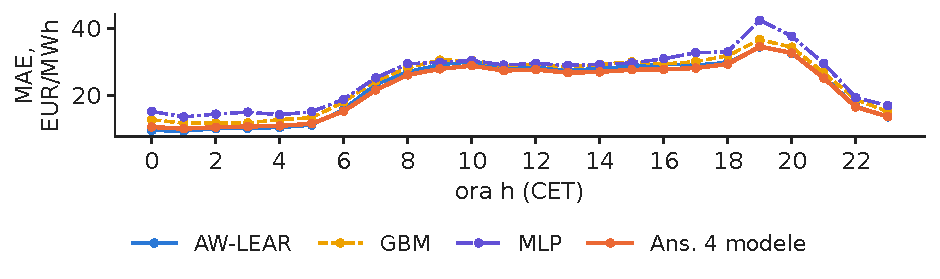
\includegraphics[width=\textwidth,height=0.500\textheight,keepaspectratio]{charts/ro/ml_hour.pdf}\end{center}\vspace{-3mm}
\chartsource{Sursa: energy-charts.info (Fraunhofer ISE); prețuri OPCOM; producție și fluxuri ENTSO-E (date Transelectrica pentru România); Yahoo Finance (SparkChange EUA ETC). Date: anul de test 2025-11-01 - 2026-10-31; modelele ML reestimate lunar.}
\vspace{0.5mm}
\begin{itemize}\setlength{\itemsep}{0pt}
  \item GBM este mai precis decît AW-LEAR în 0 ore, MLP în 0, iar ansamblul de 4 modele în 15 din 24 de ore.
  \item Ora cea mai dificilă este 19 CET, cînd prețul urcă abrupt seara (MAE AW-LEAR 34{,}52 EUR/MWh).
\end{itemize}
\par\vfill\manager{alocați cel mai bun analist orelor de seară, unde se pierd cei mai mulți bani.}\par\vspace{0.5mm}
\par\vfill\noindent{\scriptsize\color{FooterGray}(calcule proprii, anul de test 1 noiembrie 2025 -- 31 octombrie 2026)}\hfill\qlink{EMQA\_L2\_ml\_hour}{Quantlets/L2/EMQA_L2_ml_hour}\par\vspace{0.5mm}
\end{frame}

\begin{frame}{Studiul de caz C2: pentru consumul din România, învățarea automată dă cele mai mici erori}
\footnotesize
\begin{itemize}\setlength{\itemsep}{1pt}
  \item \textbf{Ce a făcut lucrarea} (Proșcanu, Proșcanu, Pele \& Costea, 2025)
    \begin{itemize}\setlength{\itemsep}{0pt}
      \item Date și metode: consumul național orar al României, 2022--2024; modele sezoniere clasice comparate cu rețele neuronale
      \item Rezultat: o rețea neuronală are o eroare net mai mică decît modelul autoregresiv sezonier
    \end{itemize}
  \item \textbf{Replicarea noastră} (studiul de caz C2, cu aceeași regulă: date pînă la 12:00 în ziua $d-1$)
    \begin{itemize}\setlength{\itemsep}{0pt}
      \item 217 zile de test, începînd cu 27 mai 2024; consumul măsurat pînă în ziua $d-2$
      \item MAPE: gradient boosting 4{,}09\%, modelul fundațional Chronos-Bolt 4{,}16\%, MLP 4{,}58\%
      \item Regresie liniară 4{,}85\%, model autoregresiv sezonier 8{,}03\%, modelul naiv (consumul de acum două zile) 10{,}17\%
    \end{itemize}
  \item \textbf{De ce rezultatul diferă de cel pentru prețuri}
    \begin{itemize}\setlength{\itemsep}{0pt}
      \item Consumul variază lin și nu se apropie de zero: MAPE are sens, iar modelele neliniare găsesc regularități
      \item Prețurile au salturi și devin negative: aici, un model liniar bine construit este greu de depășit
    \end{itemize}
\end{itemize}
\par\vspace{0.5mm}{\scriptsize \begin{itemize}\setlength{\itemsep}{0pt}
  \item Cifrele C2 sînt calculate cu notebook-ul Jupyter al studiului de caz C2, pe datele noastre; rezultatele lucrării sînt prezentate în fișa studiului de caz.
\end{itemize}}
\par\vfill\manager{prognozați consumul propriu cu modele ML, iar prețul cu LEAR și un ansamblu de modele.}\par\vspace{0.5mm}
\par\vfill\noindent{\scriptsize\color{FooterGray}(Proșcanu, Proșcanu, Pele \& Costea, 2025, RJEF; studiul de caz C2)}\par\vspace{0.5mm}
\end{frame}


\section{Prognoze probabilistice și cointegrare}

\subsection{Medierea prin regresie cuantilică}

\begin{frame}{Medierea prin regresie cuantilică: de la prognoze punctuale la cuantile}
\footnotesize
\intuition{Regresăm prețul realizat pe mai multe prognoze punctuale, separat pentru fiecare nivel al cuantilei; rezultatul este o distribuție a prețului.}
\begin{columns}[T,onlytextwidth]
\begin{column}{0.52\textwidth}
\[ \hat q^{\tau}_{d,h}=\beta^{\tau}_{0,h}+\beta^{\tau}_{1,h}\hat P^{\text{AW-ARX}}_{d,h}+\beta^{\tau}_{2,h}\hat P^{\text{AW-LEAR}}_{d,h} \]\[ \text{PS}_\tau(q,y)=\big(\mathbb 1\{y<q\}-\tau\big)(q-y) \]{\footnotesize\begin{itemize}\setlength{\itemsep}{0pt}
  \item \textbf{\txtwhere}
    \begin{itemize}\setlength{\itemsep}{0pt}
      \item $\hat q^{\tau}_{d,h}$ = cuantila de nivel $\tau$ a prețului
      \item $\bm\beta^{\tau}_h$ minimizează scorul pinball (PS) pe prognozele din ultimele 182 de zile, cu reestimare săptămînală
      \item $\tau=0{,}01,\dots,0{,}99$.
    \end{itemize}
\end{itemize}\par}
\end{column}
\begin{column}{0.45\textwidth}
\begin{itemize}\setlength{\itemsep}{1pt}
  \item \textbf{Pe datele din România}, scorul pinball mediu (mai mic = mai bine)
    \begin{itemize}\setlength{\itemsep}{0pt}
      \item QRA 8{,}33; predicție conformală (CP) 8{,}47; simulare istorică (HS) 8{,}41
      \item CP și HS folosesc erorile AW-LEAR din ultimele 112 zile, ca în tema 1
    \end{itemize}
  \item \textbf{Acoperirea intervalului de 90\%}
    \begin{itemize}\setlength{\itemsep}{0pt}
      \item QRA 85{,}7\%, CP 87{,}0\%, HS 85{,}8\%; lățimea medie a intervalului QRA: 93{,}0 EUR/MWh
      \item Toate sub 90\%; testul Kupiec respinge ipoteza unei acoperiri corecte
    \end{itemize}
\end{itemize}
\end{column}
\end{columns}
\par\vfill\manager{o bandă de 90\% care conține doar 86\% din prețuri subestimează riscul poziției deschise.}\par\vspace{0.5mm}
\par\vfill\noindent{\scriptsize\color{FooterGray}(Koenker \& Bassett, 1978; Nowotarski \& Weron, 2015)}\hfill\tryit{notebook-ul Jupyter, secțiunea 7}\par\vspace{0.5mm}
\end{frame}

\begin{frame}{O săptămînă de intervale QRA în România: largi seara, înguste noaptea}
\small
\begin{center}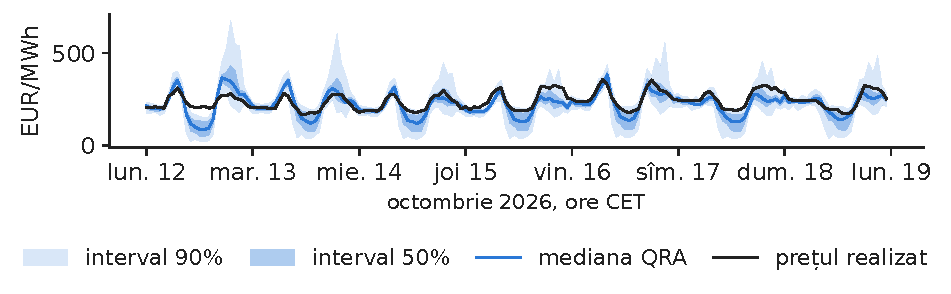
\includegraphics[width=\textwidth,height=0.399\textheight,keepaspectratio]{charts/ro/qra_week.pdf}\end{center}\vspace{-3mm}
\chartsource{Sursa: energy-charts.info (Fraunhofer ISE); prețuri OPCOM; consum, producție eoliană și solară ENTSO-E (date Transelectrica pentru România). Date: săptămîna 2026-10-12 - 2026-10-18, date orare.}
\vspace{0.5mm}
\begin{itemize}\setlength{\itemsep}{0pt}
  \item Săptămîna 12 octombrie 2026 -- 18 octombrie 2026
    \begin{itemize}\setlength{\itemsep}{0pt}
      \item Intervalul se lărgește seara, cînd prețul este incert, și se îngustează noaptea, cînd prețul este stabil.
    \end{itemize}
  \item Mediana QRA are MAE 22{,}14 EUR/MWh, la fel de precisă ca cea mai bună prognoză punctuală.
\end{itemize}
\par\vfill\manager{pentru volumele pe care trebuie să le cumpărați, ofertați în intervalul de 50\%
    \begin{itemize}\setlength{\itemsep}{0pt}
      \item Pentru cele pe care le puteți muta în altă oră, folosiți cozile.
    \end{itemize}}\par\vspace{0.5mm}
\par\vfill\noindent{\scriptsize\color{FooterGray}(Nowotarski \& Weron, 2015, Comput.\ Stat.)}\hfill\qlink{EMQA\_L2\_qra\_week}{Quantlets/L2/EMQA_L2_qra_week}\par\vspace{0.5mm}
\end{frame}

\begin{frame}{Toate cele trei metode subestimează cozile distribuției prețului}
\small
\begin{center}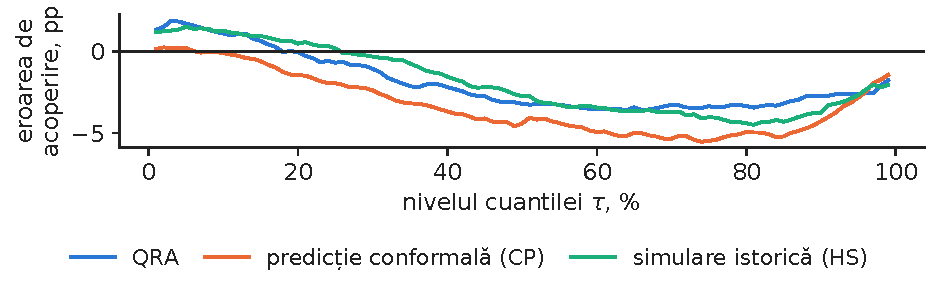
\includegraphics[width=\textwidth,height=0.405\textheight,keepaspectratio]{charts/ro/prob_rel.pdf}\end{center}\vspace{-3mm}
\chartsource{Sursa: energy-charts.info (Fraunhofer ISE); prețuri OPCOM; consum, producție eoliană și solară ENTSO-E (date Transelectrica pentru România). Date: anul de test 2025-11-01 - 2026-10-31, 99 de cuantile.}
\vspace{0.5mm}
\begin{itemize}\setlength{\itemsep}{0pt}
  \item Calibrare perfectă = exact $\tau$\% din prețuri sub cuantila de nivel $\tau$ (linia 0)
    \begin{itemize}\setlength{\itemsep}{0pt}
      \item Peste linie în stînga și sub linie în dreapta = cozi prea înguste.
    \end{itemize}
  \item Statistica Kupiec pentru intervalul de 90\%: QRA 162{,}9, CP 83{,}3, HS 154{,}1 (valoarea critică la 5\% este 3{,}84).
\end{itemize}
\par\vfill\manager{lărgiți cozile înainte de a folosi cuantilele pentru calculul garanțiilor (cursul 4).}\par\vspace{0.5mm}
\par\vfill\noindent{\scriptsize\color{FooterGray}(Kupiec, 1995, J.\ Derivatives; Gneiting \& Raftery, 2007, JASA)}\hfill\qlink{EMQA\_L2\_prob\_rel}{Quantlets/L2/EMQA_L2_prob_rel}\par\vspace{0.5mm}
\end{frame}

\subsection{Cointegrarea: prețuri care evoluează împreună}

\begin{frame}{Două prețuri sînt cointegrate dacă diferența dintre ele revine spre echilibru}
\footnotesize
\intuition{Fiecare preț poate fi nestaționar, dar, dacă o combinație liniară a lor este staționară, abaterea se închide, iar regresia nu este spurioasă.}
\begin{columns}[T,onlytextwidth]
\begin{column}{0.50\textwidth}
\[ \underbrace{P^{\text{RO}}_t=\alpha+\beta P^{\text{HU}}_t+u_t}_{\text{pasul 1, OLS}} \]\vspace{-2mm}\[ \underbrace{\Delta\hat u_t=\rho\,\hat u_{t-1}+\textstyle\sum_j\gamma_j\Delta\hat u_{t-j}+\eta_t}_{\text{pasul 2, rădăcină unitară în } \hat u} \]{\footnotesize\begin{itemize}\setlength{\itemsep}{0pt}
  \item \textbf{\txtwhere}
    \begin{itemize}\setlength{\itemsep}{0pt}
      \item Engle--Granger: $H_0$ = fără cointegrare ($\rho=0$), valori critice MacKinnon
      \item Johansen: testul urmei pentru rangul $r$ (numărul relațiilor de cointegrare).
    \end{itemize}
\end{itemize}\par}
\end{column}
\begin{column}{0.47\textwidth}
\begin{itemize}\setlength{\itemsep}{1pt}
  \item \textbf{România și Ungaria}, zilnic, din 1 ianuarie 2022
    \begin{itemize}\setlength{\itemsep}{0pt}
      \item $\hat\beta$ = 0{,}963; Engle--Granger \ensuremath{-}10{,}58 (critic la 5\%: \ensuremath{-}3{,}34): cointegrate
      \item Un șoc asupra diferenței de preț se înjumătățește în 0{,}8 zile
    \end{itemize}
  \item \textbf{Testul urmei Johansen}
    \begin{itemize}\setlength{\itemsep}{0pt}
      \item $r=0$: 139{,}7 față de 15{,}49; $r\le1$: 6{,}21 față de 3{,}84
      \item Rangul 2: nivelurile sînt aproape staționare din 2022 (testul Dickey--Fuller augmentat (ADF), $p$ = 0{,}064)
    \end{itemize}
\end{itemize}
\end{column}
\end{columns}
\par\vfill\manager{o poziție pe diferența de preț RO--HU se închide în cîteva zile, nu în luni.}\par\vspace{0.5mm}
\par\vfill\noindent{\scriptsize\color{FooterGray}(Engle \& Granger, 1987; Johansen, 1991; MacKinnon, 1996)}\hfill\tryit{notebook-ul Jupyter, secțiunea 8}\par\vspace{0.5mm}
\end{frame}

\begin{frame}{România și Ungaria: piețe cuplate, cu o diferență de preț care se închide repede}
\small
\begin{center}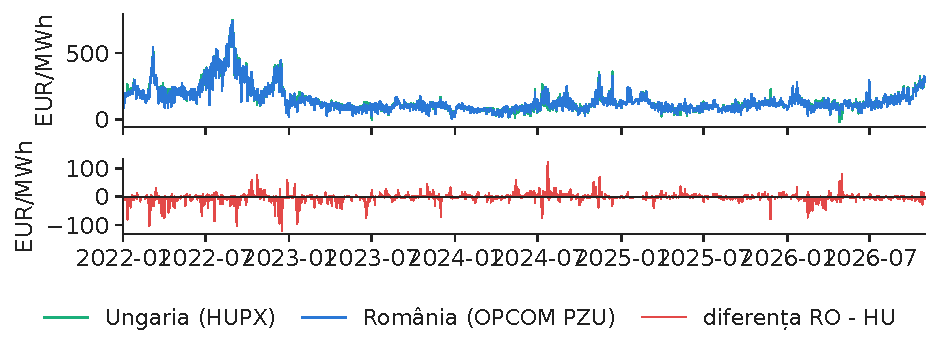
\includegraphics[width=\textwidth,height=0.425\textheight,keepaspectratio]{charts/ro/coint_daily.pdf}\end{center}\vspace{-3mm}
\chartsource{Sursa: energy-charts.info (Fraunhofer ISE); prețurile OPCOM (RO), HUPX (HU) și EPEX SPOT (DE-LU), prin ENTSO-E. Date: prețuri zilnice de bază, 2022-01-01 - 2026-10-31.}
\vspace{0.5mm}
\begin{itemize}\setlength{\itemsep}{0pt}
  \item Diferența RO $-$ HU: media \ensuremath{-}2{,}07, abaterea standard 15{,}08 EUR/MWh
    \begin{itemize}\setlength{\itemsep}{0pt}
      \item Pentru România și Germania--Luxemburg: 21{,}06 și 37{,}79.
    \end{itemize}
  \item În anul de test, prețurile din RO și HU au fost identice în 10{,}1\% din ore
    \begin{itemize}\setlength{\itemsep}{0pt}
      \item În restul orelor, interconexiunea a fost congestionată.
    \end{itemize}
\end{itemize}
\par\vfill\manager{folosiți prețul din Ungaria ca regresor sau ca verificare a prognozei pentru România.}\par\vspace{0.5mm}
\par\vfill\noindent{\scriptsize\color{FooterGray}(Engle \& Granger, 1987, Econometrica)}\hfill\qlink{EMQA\_L2\_coint\_daily}{Quantlets/L2/EMQA_L2_coint_daily}\par\vspace{0.5mm}
\end{frame}

\begin{frame}{Prețul energiei revine spre nivelul dat de gaze: model cu corecția erorii}
\footnotesize
\intuition{Dacă prețurile energiei și gazelor sînt cointegrate, prețul energiei revine lunar spre nivelul dat de gaze, iar producția hidro îl abate temporar.}
\begin{columns}[T,onlytextwidth]
\begin{column}{0.53\textwidth}
\[ \Delta P_t=c+\underbrace{\alpha\,(P_{t-1}-a-\beta\,\text{TTF}_{t-1})}_{\text{corecția erorii}}+\gamma\,\Delta\text{TTF}_t+\delta\,H_t+\varepsilon_t \]{\footnotesize\begin{itemize}\setlength{\itemsep}{0pt}
  \item \textbf{\txtwhere}
    \begin{itemize}\setlength{\itemsep}{0pt}
      \item $P_t$ = prețul mediu lunar al energiei electrice din România
      \item TTF = prețul gazelor, în EUR/MWh
      \item $H_t$ = producția hidro minus media lunii calendaristice (TWh), staționară
      \item $\alpha<0$ = viteza de revenire spre echilibru.
    \end{itemize}
\end{itemize}\par}
\end{column}
\begin{column}{0.44\textwidth}
\begin{itemize}\setlength{\itemsep}{1pt}
  \item \textbf{Pe datele din România}, 2015-01 -- 2026-10
    \begin{itemize}\setlength{\itemsep}{0pt}
      \item Engle--Granger \ensuremath{-}5{,}64 (valoarea critică la 5\%: \ensuremath{-}3{,}38); rangul Johansen: 1
      \item $\hat\beta$ = 1{,}95, ca și cum prețul ar fi stabilit de o centrală pe gaze cu randament de circa 51\%
    \end{itemize}
  \item \textbf{Modelul cu corecția erorii (ECM)}
    \begin{itemize}\setlength{\itemsep}{0pt}
      \item $\hat\alpha$ = \ensuremath{-}0{,}452; timpul de înjumătățire: 1{,}2 luni
      \item $\hat\delta$ = \ensuremath{-}12{,}80 EUR/MWh pentru fiecare TWh suplimentar de producție hidro ($t$ = \ensuremath{-}3{,}10)
    \end{itemize}
\end{itemize}
\end{column}
\end{columns}
\par\vfill\manager{într-o lună secetoasă, un producător hidro se poate aștepta la prețuri peste nivelul dat de gaze timp de una sau două luni.}\par\vspace{0.5mm}
\par\vfill\noindent{\scriptsize\color{FooterGray}(Engle \& Granger, 1987; Johansen, 1991, Econometrica)}\hfill\tryit{notebook-ul Jupyter, secțiunea 8}\par\vspace{0.5mm}
\end{frame}

\begin{frame}{Prețul energiei, gazele și hidro: regresia din cursul 1 nu este spurioasă}
\small
\begin{center}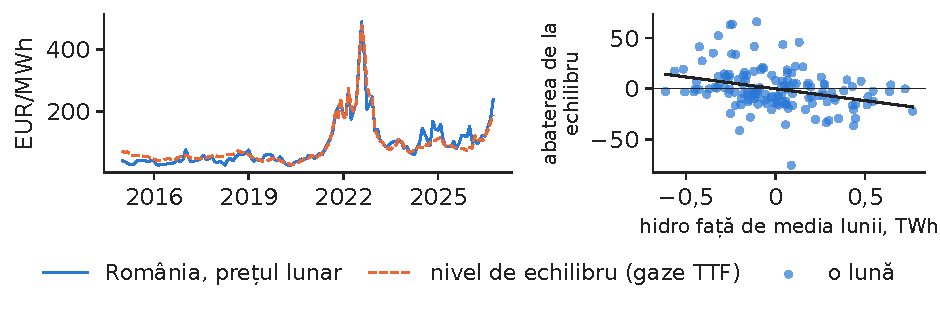
\includegraphics[width=\textwidth,height=0.436\textheight,keepaspectratio]{charts/ro/coint_monthly.pdf}\end{center}\vspace{-3mm}
\chartsource{Sursa: energy-charts.info (prețuri OPCOM; producția hidro ENTSO-E, date Transelectrica); Banca Mondială, Pink Sheet (TTF). Date: lunar, 2015-01 - 2026-10.}
\vspace{0.5mm}
\begin{itemize}\setlength{\itemsep}{0pt}
  \item În stînga, prețul lunar urmează nivelul de echilibru dat de prețul gazelor
    \begin{itemize}\setlength{\itemsep}{0pt}
      \item În dreapta, în lunile cu producție hidro peste medie, prețul este sub acest nivel.
    \end{itemize}
\end{itemize}
\par\vfill\manager{interpretați un an hidrologic secetos ca o primă de preț peste nivelul dat de gaze, nu ca un nou nivel al prețului.}\par\vspace{0.5mm}
\par\vfill\noindent{\scriptsize\color{FooterGray}(cursul 1, studiul de caz hidro; estimare proprie)}\hfill\qlink{EMQA\_L2\_coint\_monthly}{Quantlets/L2/EMQA_L2_coint_monthly}\par\vspace{0.5mm}
\end{frame}


\section{Studii de caz pe date recente din România}

\subsection{(a) Un an de prognoze}

\begin{frame}{Studiul de caz (a): acuratețea diferă mult de la o lună la alta}
\small
\begin{center}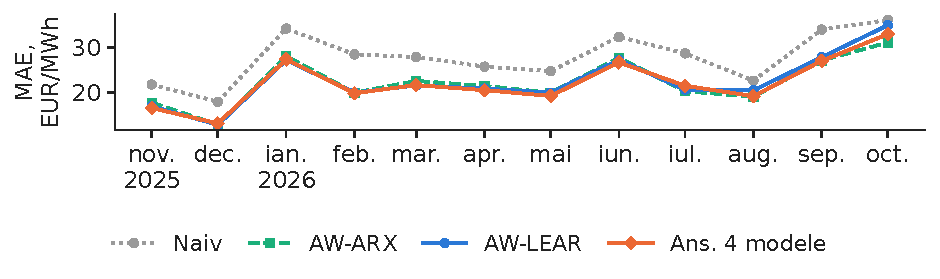
\includegraphics[width=\textwidth,height=0.500\textheight,keepaspectratio]{charts/ro/monthly_mae.pdf}\end{center}\vspace{-3mm}
\chartsource{Sursa: energy-charts.info (Fraunhofer ISE); prețuri OPCOM; producție și fluxuri ENTSO-E (date Transelectrica pentru România); Yahoo Finance (SparkChange EUA ETC). Date: anul de test 2025-11-01 - 2026-10-31.}
\vspace{0.5mm}
\begin{itemize}\setlength{\itemsep}{0pt}
  \item AW-LEAR este mai precis decît modelul naiv în 12 din 12 luni
    \begin{itemize}\setlength{\itemsep}{0pt}
      \item MAE variază între 12{,}84 (decembrie 2025) și 34{,}88 EUR/MWh (octombrie 2026).
    \end{itemize}
\end{itemize}
\par\vfill\manager{raportați acuratețea lună de lună: o MAE anuală bună poate ascunde o toamnă slabă.}\par\vspace{0.5mm}
\par\vfill\noindent{\scriptsize\color{FooterGray}(calcule proprii, anul de test 1 noiembrie 2025 -- 31 octombrie 2026)}\hfill\qlink{EMQA\_L2\_monthly\_mae}{Quantlets/L2/EMQA_L2_monthly_mae}\par\vspace{0.5mm}
\end{frame}

\subsection{(b) O săptămînă de criză}

\begin{frame}{Studiul de caz (b): în săptămîna de criză (19 octombrie 2026) modelele întîrzie o zi}
\small
\begin{center}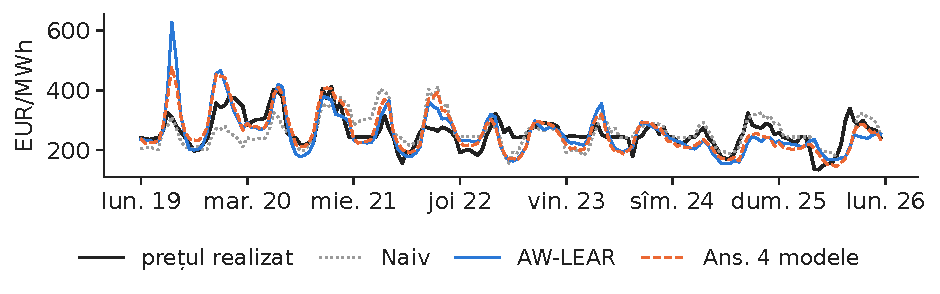
\includegraphics[width=\textwidth,height=0.398\textheight,keepaspectratio]{charts/ro/stress_week.pdf}\end{center}\vspace{-3mm}
\chartsource{Sursa: energy-charts.info (Fraunhofer ISE); prețuri OPCOM; producție și fluxuri ENTSO-E (date Transelectrica pentru România); Yahoo Finance (SparkChange EUA ETC). Date: săptămîna 2026-10-19 - 2026-10-25, date orare.}
\vspace{0.5mm}
\begin{itemize}\setlength{\itemsep}{0pt}
  \item Prețul mediu 258{,}59, maximul 412{,}35 EUR/MWh
    \begin{itemize}\setlength{\itemsep}{0pt}
      \item MAE: modelul naiv 40{,}19, AW-LEAR 36{,}54, GBM 34{,}35, ansamblul 34{,}95.
    \end{itemize}
\end{itemize}
\par\vfill\manager{toate modelele reacționează la un salt de nivel cu o zi întîrziere
    \begin{itemize}\setlength{\itemsep}{0pt}
      \item Acoperiți riscul orelor de seară.
    \end{itemize}}\par\vspace{0.5mm}
\par\vfill\noindent{\scriptsize\color{FooterGray}(calcule proprii; OPCOM)}\hfill\qlink{EMQA\_L2\_stress\_week}{Quantlets/L2/EMQA_L2_stress_week}\par\vspace{0.5mm}
\end{frame}

\subsection{(c) Intervalul de tranzacționare de 15 minute}

\begin{frame}{Studiul de caz (c): sferturile de oră cer un profil în interiorul orei}
\small
\begin{center}
\includegraphics[width=\textwidth,height=0.326\textheight,keepaspectratio]{charts/ro/mtu15.pdf}\end{center}\vspace{-3mm}
\chartsource{Sursa: energy-charts.info (Fraunhofer ISE); prețurile PZU pe 15 minute ale OPCOM pentru România, prin ENTSO-E. Date: 2026-07-01, 96 de sferturi de oră (CET).}
\vspace{0.5mm}
\begin{itemize}\setlength{\itemsep}{0pt}
  \item Intervalul de tranzacționare (MTU) are 15 minute
    \begin{itemize}\setlength{\itemsep}{0pt}
      \item Prognoza = AW-LEAR orar + profilul intraorar mediu din ultimele 28 de zile.
    \end{itemize}
  \item 363 de zile fără schimbarea orei
    \begin{itemize}\setlength{\itemsep}{0pt}
      \item MAE pe sfert de oră: 26{,}02 constant în oră, 24{,}53 EUR/MWh cu profil.
    \end{itemize}
\end{itemize}
\par\vfill\manager{o baterie licitează pe sferturi de oră
    \begin{itemize}\setlength{\itemsep}{0pt}
      \item Folosiți profilul intraorar, nu o valoare constantă.
    \end{itemize}}\par\vspace{0.5mm}
\par\vfill\noindent{\scriptsize\color{FooterGray}(calcule proprii; OPCOM; trecerea SDAC la 15 minute, 1 oct. 2025)}\hfill\qlink{EMQA\_L2\_mtu15}{Quantlets/L2/EMQA_L2_mtu15}\par\vspace{0.5mm}
\end{frame}

\subsection{(d) Valoarea economică a prognozei}

\begin{frame}{Studiul de caz (d): cît valorează, în bani, o prognoză mai bună}
\small
\begin{center}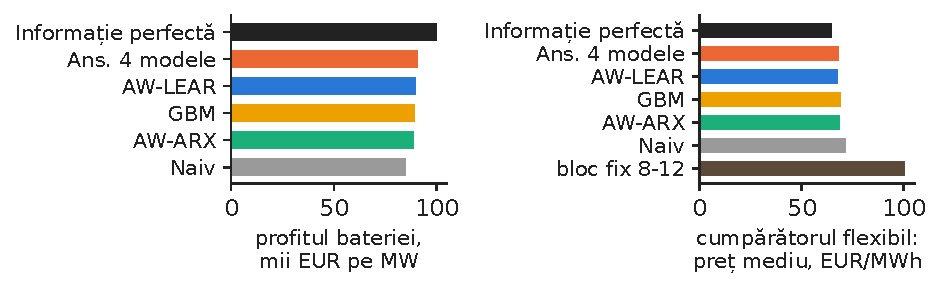
\includegraphics[width=\textwidth,height=0.373\textheight,keepaspectratio]{charts/ro/battery.pdf}\end{center}\vspace{-3mm}
\chartsource{Sursa: energy-charts.info (Fraunhofer ISE); prețuri OPCOM; producție și fluxuri ENTSO-E (date Transelectrica pentru România); Yahoo Finance (SparkChange EUA ETC). Date: anul de test 2025-11-01 - 2026-10-31; 1 MW / 2 MWh, randament 90\%.}
\vspace{0.5mm}
\begin{itemize}\setlength{\itemsep}{0pt}
  \item Baterie de 1 MW / 2 MWh, un ciclu pe zi ales după prognoză
    \begin{itemize}\setlength{\itemsep}{0pt}
      \item În 363 de zile fără schimbarea orei: 90\,738 EUR pe MW cu ansamblul (91{,}0\% din profitul cu informație perfectă), 84\,623 cu modelul naiv.
    \end{itemize}
  \item Proces flexibil de 4 ore al unui furnizor: 67{,}87 EUR/MWh cu AW-LEAR, față de 100{,}59 pentru un bloc fix 8--12 CET.
\end{itemize}
\par\vfill\manager{transformați rMAE în EUR înainte de a plăti pentru o prognoză.}\par\vspace{0.5mm}
\par\vfill\noindent{\scriptsize\color{FooterGray}(calcule proprii; randament de încărcare--descărcare presupus: 90\%)}\hfill\qlink{EMQA\_L2\_battery}{Quantlets/L2/EMQA_L2_battery}\par\vspace{0.5mm}
\end{frame}

\begin{frame}{O prognoză se acceptă numai după o listă de verificări; testul nostru arată că nu folosim informație din viitor}
\footnotesize
\begin{columns}[T,onlytextwidth]
\begin{column}{0.52\textwidth}
\begin{itemize}\setlength{\itemsep}{1pt}
  \item \textbf{Înainte să aveți încredere într-o testare retrospectivă}
    \begin{itemize}\setlength{\itemsep}{0pt}
      \item Fiecare variabilă de intrare este publicată înainte de ora 12:00 CET din ziua $d-1$
      \item Standardizările, transformările, $\lambda$ și pragurile se estimează numai pe fereastra de calibrare
      \item Validarea este cronologică, iar anul de test este folosit o singură dată
    \end{itemize}
  \item \textbf{Apoi raportați}
    \begin{itemize}\setlength{\itemsep}{0pt}
      \item MAE și rMAE față de modelul naiv, valorile $p$ ale testelor DM, acoperirea intervalelor
      \item Rezultate pe luni și pe ore, nu doar o cifră anuală
    \end{itemize}
\end{itemize}
\end{column}
\begin{column}{0.45\textwidth}
\begin{itemize}\setlength{\itemsep}{1pt}
  \item \textbf{Autoverificarea noastră} (scriptul de analiză, secțiunea 7)
    \begin{itemize}\setlength{\itemsep}{0pt}
      \item 9\,364 de verificări ale momentului publicării: fiecare variabilă este disponibilă cu cel puțin 12 h înainte de ora 12:00
      \item 17 serii de prognoză recalculate în 14 zile; GBM și MLP, în prima zi a fiecăreia dintre cele 12 reestimări
      \item Datele ulterioare au fost șterse sau înlocuite cu valori absurde: prognozele au rămas identice, pînă la rotunjire
      \item Rezultat: verificare trecută
    \end{itemize}
\end{itemize}
\end{column}
\end{columns}
\par\vfill\manager{includeți testul de folosire a informației din viitor în orice evaluare a unui model, ca în tema 1.}\par\vspace{0.5mm}
\par\vfill\noindent{\scriptsize\color{FooterGray}(tema 1; Lago et al., 2021, APEN)}\hfill\tryit{notebook-ul Jupyter, secțiunea 10}\par\vspace{0.5mm}
\end{frame}

\section*{Recapitulare}

\begin{frame}{Test 1: modelul naiv pentru o zi de luni}
\small
\begin{itemize}
  \item Este duminică, ora 11:30 CET
    \begin{itemize}\setlength{\itemsep}{0pt}
      \item Trebuie să prognozați cu modelul naiv prețul de luni pentru ora 19:00
      \item Ce preț folosiți?
    \end{itemize}
\end{itemize}
\vspace{2mm}
\begin{exampleblock}{R\u{a}spuns}
\begin{itemize}
  \item Prețul de luni trecută, ora 19:00 ($d-7$)
    \begin{itemize}\setlength{\itemsep}{0pt}
      \item În anul de test, pentru zilele de luni, sîmbătă și duminică, această regulă este mai precisă decît prețul din ziua precedentă (MAE 29{,}87 față de 33{,}48 EUR/MWh).
    \end{itemize}
\end{itemize}
\end{exampleblock}
\end{frame}

\begin{frame}{Test 2: o testare retrospectivă suspectă}
\small
\begin{itemize}
  \item Un furnizor de prognoze raportează rMAE 0{,}55 pentru România, dar folosește ca regresor consumul realizat în ziua $d-1$
    \begin{itemize}\setlength{\itemsep}{0pt}
      \item Cumpărați prognoza?
    \end{itemize}
\end{itemize}
\vspace{2mm}
\begin{exampleblock}{R\u{a}spuns}
\begin{itemize}
  \item Nu: la ora 12:00 din ziua $d-1$, consumul acelei zile nu este încă măsurat, deci testarea folosește informație din viitor
    \begin{itemize}\setlength{\itemsep}{0pt}
      \item Cereți o nouă testare cu date pînă în ziua $d-2$ (sau cu prognozele publicate de TSO)
      \item Cel mai bun rezultat corect al nostru este rMAE 0{,}795.
    \end{itemize}
\end{itemize}
\end{exampleblock}
\end{frame}

\begin{frame}{Test 3: interpretarea testului DM}
\small
\begin{itemize}
  \item AW-LEAR sau AW-ARX? Testul DM dă $p$ = 0{,}797
    \begin{itemize}\setlength{\itemsep}{0pt}
      \item Ce model intră în producție?
    \end{itemize}
\end{itemize}
\vspace{2mm}
\begin{exampleblock}{R\u{a}spuns}
\begin{itemize}
  \item Niciunul nu este semnificativ mai precis
    \begin{itemize}\setlength{\itemsep}{0pt}
      \item Alegeți modelul mai simplu sau, mai bine, media lor, care face parte din cel mai bun ansamblu (rMAE 0{,}795).
    \end{itemize}
\end{itemize}
\end{exampleblock}
\end{frame}

\begin{frame}{Test 4: o măsură a erorii pentru consiliul de administrație}
\small
\begin{itemize}
  \item Raportul dumneavoastră indică MAPE 5\,778\% pentru prognoza prețului din România, iar consiliul este alarmat
    \begin{itemize}\setlength{\itemsep}{0pt}
      \item Ce răspundeți?
    \end{itemize}
\end{itemize}
\vspace{2mm}
\begin{exampleblock}{R\u{a}spuns}
\begin{itemize}
  \item MAPE împarte eroarea la prețuri apropiate de zero (387 de ore sub 5 EUR/MWh produc 99{,}5\% din valoarea ei)
    \begin{itemize}\setlength{\itemsep}{0pt}
      \item Raportați în schimb MAE 22{,}53 EUR/MWh și rMAE 0{,}810.
    \end{itemize}
\end{itemize}
\end{exampleblock}
\end{frame}

\begin{frame}{Test 5: cointegrarea în practică}
\small
\begin{itemize}
  \item Prețurile din România și Ungaria sînt cointegrate, iar un șoc asupra diferenței se înjumătățește în 0{,}8 zile
    \begin{itemize}\setlength{\itemsep}{0pt}
      \item Astăzi prețul din România este cu 40 EUR/MWh mai mare decît cel din Ungaria
      \item La ce vă așteptați?
    \end{itemize}
\end{itemize}
\vspace{2mm}
\begin{exampleblock}{R\u{a}spuns}
\begin{itemize}
  \item Diferența ar trebui să se reducă la circa jumătate în aproximativ o zi, dacă interconexiunea nu rămîne congestionată
    \begin{itemize}\setlength{\itemsep}{0pt}
      \item Este un semnal pentru tranzacțiile transfrontaliere, nu o garanție.
    \end{itemize}
\end{itemize}
\end{exampleblock}
\end{frame}

\begin{frame}{Recapitulare}
\small
\vspace{-2mm}\begin{multicols}{2}\scriptsize\tableofcontents\end{multicols}
\begin{itemize}\setlength{\itemsep}{1pt}
  \item Mai întîi, un cadru corect: numai informația disponibilă la ora 12:00 CET în ziua $d-1$, ferestre glisante, modelul naiv ca reper și teste DM.
  \item În anul de test, cel mai bun model, ansamblul de 4 modele, reduce eroarea modelului naiv cu 20{,}5\%
    \begin{itemize}\setlength{\itemsep}{0pt}
      \item Cursul următor: volatilitatea (cursul 3).
    \end{itemize}
\end{itemize}
\end{frame}

\begin{frame}{Cercetările grupului nostru despre prognoza consumului și a prețurilor în România}
\footnotesize
\begin{itemize}\setlength{\itemsep}{1pt}
  \item \textbf{Compararea modelelor de prognoză a consumului} (Proșcanu, Proșcanu, Pele \& Costea, 2025, RJEF)
    \begin{itemize}\setlength{\itemsep}{0pt}
      \item Ce a făcut lucrarea: a comparat modele sezoniere clasice și rețele neuronale pe consumul național orar al României
      \item Rezultat: o rețea neuronală are o eroare net mai mică decît modelul autoregresiv sezonier (studiul de caz C2)
    \end{itemize}
  \item \textbf{Patru generații de modele pentru prețul energiei} (Andrei, Velev, Toma, Pele \& Lessmann, 2024, arXiv 2411.03372)
    \begin{itemize}\setlength{\itemsep}{0pt}
      \item Ce a făcut lucrarea: a evaluat comparativ patru generații de metode de prognoză a prețurilor energiei
      \item Utilitate: un reper pentru alegerea familiei de modele
    \end{itemize}
  \item \textbf{Explicarea prognozelor de preț pe mai multe orizonturi} (Andrei, Pele \& Cramer, 2026, PICBE)
    \begin{itemize}\setlength{\itemsep}{0pt}
      \item Ce a făcut lucrarea: a explicat prognozele prețurilor orare din România
      \item Rezultat: arată ce factori contează la fiecare orizont de prognoză și în fiecare regim de preț
    \end{itemize}
  \item \textbf{Avertizarea timpurie a salturilor de preț} (Andrei, Pele, Cramer, Amza \& Diaconu, 2026, PICBE)
    \begin{itemize}\setlength{\itemsep}{0pt}
      \item Ce a făcut lucrarea: a construit un sistem explicabil de inteligență artificială (AI) pentru piața din România
      \item Rezultat: prețul anterior și consumul rezidual sînt principalii factori ai salturilor (tema cursului 7)
    \end{itemize}
\end{itemize}
\par\vspace{0.5mm}{\scriptsize \begin{itemize}\setlength{\itemsep}{0pt}
  \item Rezultatele de pe acest diapozitiv sînt cele raportate în lucrări; celelalte cifre din curs provin din calculele noastre.
\end{itemize}}
\par\vfill\noindent{\scriptsize\color{FooterGray}(Academia de Studii Economice din București; Academia Română, Institutul de Prognoză Economică)}\par\vspace{0.5mm}
\end{frame}

\begin{frame}{Lecturi și resurse suplimentare}
\small
\begin{columns}[T,onlytextwidth]
\begin{column}{0.52\textwidth}
\begin{itemize}\setlength{\itemsep}{1pt}
  \item \textbf{R.\ Weron, IIF Distinguished Lectures despre prognoza prețurilor energiei electrice} (2025): prezentări \href{https://p.wz.pwr.edu.pl/~weron.rafal/assets/PDF/Weron25_IIF_1.pdf}{partea I}, \href{https://p.wz.pwr.edu.pl/~weron.rafal/assets/PDF/Weron25_IIF_2.pdf}{partea a II-a}, \href{https://github.com/lipiecki/energy-analytics-2025}{notebook-uri Jupyter}.
  \item \textbf{epftoolbox}, LEAR și DNN, cu setul de date pentru evaluare publicat de Lago et al.\ (2021): \href{https://github.com/jeslago/epftoolbox}{github.com/jeslago/epftoolbox}.
  \item \textbf{Forecasting -- Principles and Practice}, ed.\ a 3-a, \href{https://otexts.com/fpp3/}{otexts.com/fpp3}.
\end{itemize}
\end{column}
\begin{column}{0.45\textwidth}
\begin{itemize}\setlength{\itemsep}{1pt}
  \item \textbf{Acest curs}: cod, date, notebook-uri Jupyter --- \href{https://github.com/danpele/EMQA}{github.com/danpele/EMQA}.
  \item \textbf{Tema 1} aplică ARX, LEAR, DM și intervalele HS/CP pe propria fereastră de test.
  \item \textbf{Exercițiu practic}: notebook-ul Jupyter reproduce toate graficele și cifrele din acest curs --- \href{\emqarepo/\emqanb}{notebooks/}.
\end{itemize}
\end{column}
\end{columns}
\end{frame}

\begin{frame}{Bibliografie (1/3)}
\scriptsize
\begin{itemize}\setlength{\itemsep}{1pt}\scriptsize
\item Andrei, A.-V., Pele, D.-T.\ \& Cramer, A.-A.\ (2026). Multi-horizon explainability in energy price forecasting: Disentangling market dynamics and renewable intermittency in Romania's liberalized electricity market. \textit{Proceedings of the International Conference on Business Excellence}, 20(1), 104--117. \href{https://doi.org/10.2478/picbe-2026-0014}{doi:10.2478/picbe-2026-0014}
\item Andrei, A.-V., Pele, D.-T., Cramer, A.-A., Amza, A.\ \& Diaconu, D.\ (2026). Explainable AI-based early warning system for electricity price spikes: Evidence from the Romanian market. \textit{Proceedings of the International Conference on Business Excellence}, 20(1), 4820--4836. \href{https://doi.org/10.2478/picbe-2026-0352}{doi:10.2478/picbe-2026-0352}
\item Andrei, A.-V., Velev, G., Toma, F.-M., Pele, D.\,T.\ \& Lessmann, S.\ (2024). Energy price modelling: A comparative evaluation of four generations of forecasting methods. arXiv:2411.03372.
\item Bates, J.\,M.\ \& Granger, C.\,W.\,J.\ (1969). The combination of forecasts. \textit{Operational Research Quarterly}, 20(4), 451--468.
\item Diebold, F.\,X.\ \& Mariano, R.\,S.\ (1995). Comparing predictive accuracy. \textit{Journal of Business \& Economic Statistics}, 13(3), 253--263.
\item Engle, R.\,F.\ \& Granger, C.\,W.\,J.\ (1987). Co-integration and error correction: Representation, estimation, and testing. \textit{Econometrica}, 55(2), 251--276. \href{https://doi.org/10.2307/1913236}{doi:10.2307/1913236}
\item Friedman, J.\,H.\ (2001). Greedy function approximation: A gradient boosting machine. \textit{Annals of Statistics}, 29(5), 1189--1232. \href{https://doi.org/10.1214/aos/1013203451}{doi:10.1214/aos/1013203451}
\item Gneiting, T.\ \& Raftery, A.\,E.\ (2007). Strictly proper scoring rules, prediction, and estimation. \textit{Journal of the American Statistical Association}, 102(477), 359--378. \href{https://doi.org/10.1198/016214506000001437}{doi:10.1198/016214506000001437}
\item Hubicka, K., Marcjasz, G.\ \& Weron, R.\ (2019). A note on averaging day-ahead electricity price forecasts across calibration windows. \textit{IEEE Transactions on Sustainable Energy}, 10(1), 321--323.
\end{itemize}
\end{frame}

\begin{frame}{Bibliografie (2/3)}
\scriptsize
\begin{itemize}\setlength{\itemsep}{1pt}\scriptsize
\item Hyndman, R.\,J.\ \& Koehler, A.\,B.\ (2006). Another look at measures of forecast accuracy. \textit{International Journal of Forecasting}, 22(4), 679--688. \href{https://doi.org/10.1016/j.ijforecast.2006.03.001}{doi:10.1016/j.ijforecast.2006.03.001}
\item Johansen, S.\ (1991). Estimation and hypothesis testing of cointegration vectors in Gaussian vector autoregressive models. \textit{Econometrica}, 59(6), 1551--1580. \href{https://doi.org/10.2307/2938278}{doi:10.2307/2938278}
\item Koenker, R.\ \& Bassett, G.\ (1978). Regression quantiles. \textit{Econometrica}, 46(1), 33--50. \href{https://doi.org/10.2307/1913643}{doi:10.2307/1913643}
\item Kupiec, P.\,H.\ (1995). Techniques for verifying the accuracy of risk measurement models. \textit{Journal of Derivatives}, 3(2), 73--84.
\item Lago, J., Marcjasz, G., De Schutter, B.\ \& Weron, R.\ (2021). Forecasting day-ahead electricity prices: A review of state-of-the-art algorithms, best practices and an open-access benchmark. \textit{Applied Energy}, 293, 116983. \href{https://doi.org/10.1016/j.apenergy.2021.116983}{doi:10.1016/j.apenergy.2021.116983}
\item NEMO Committee (2025). 15-Minute MTU in SDAC was implemented. SDAC press release, 1 October 2025. \href{https://nemo-committee.eu/assets/files/15-minute-mtu-in-sdac-was-implemented.pdf}{nemo-committee.eu}
\item NEMO Committee (2026). Single Day-Ahead Coupling (SDAC) and the EUPHEMIA algorithm. \href{https://www.nemo-committee.eu/sdac}{nemo-committee.eu/sdac}
\item MacKinnon, J.\,G.\ (1996). Numerical distribution functions for unit root and cointegration tests. \textit{Journal of Applied Econometrics}, 11(6), 601--618.
\item Marcjasz, G., Serafin, T.\ \& Weron, R.\ (2018). Selection of calibration windows for day-ahead electricity price forecasting. \textit{Energies}, 11(9), 2364.
\end{itemize}
\end{frame}

\begin{frame}{Bibliografie (3/3)}
\scriptsize
\begin{itemize}\setlength{\itemsep}{1pt}\scriptsize
\item Nogales, F.\,J., Contreras, J., Conejo, A.\,J.\ \& Espínola, R.\ (2002). Forecasting next-day electricity prices by time series models. \textit{IEEE Transactions on Power Systems}, 17(2), 342--348. \href{https://doi.org/10.1109/TPWRS.2002.1007902}{doi:10.1109/TPWRS.2002.1007902}
\item Nowotarski, J.\ \& Weron, R.\ (2015). Computing electricity spot price prediction intervals using quantile regression and forecast averaging. \textit{Computational Statistics}, 30(3), 791--803. \href{https://doi.org/10.1007/s00180-014-0523-0}{doi:10.1007/s00180-014-0523-0}
\item Nowotarski, J.\ \& Weron, R.\ (2018). Recent advances in electricity price forecasting: A review of probabilistic forecasting. \textit{Renewable and Sustainable Energy Reviews}, 81, 1548--1568. \href{https://doi.org/10.1016/j.rser.2017.05.234}{doi:10.1016/j.rser.2017.05.234}
\item Proșcanu, C.\,A., Proșcanu, M.\,E., Pele, D.\,T.\ \& Costea, A.\ (2025). Watt's next? Benchmarking time series models on Romania's national electricity consumption. \textit{Romanian Journal of Economic Forecasting}, 28(3), 146--163.
\item Tibshirani, R.\ (1996). Regression shrinkage and selection via the lasso. \textit{Journal of the Royal Statistical Society B}, 58(1), 267--288. \href{https://doi.org/10.1111/j.2517-6161.1996.tb02080.x}{doi:10.1111/j.2517-6161.1996.tb02080.x}
\item Uniejewski, B., Nowotarski, J.\ \& Weron, R.\ (2016). Automated variable selection and shrinkage for day-ahead electricity price forecasting. \textit{Energies}, 9(8), 621. \href{https://doi.org/10.3390/en9080621}{doi:10.3390/en9080621}
\item Uniejewski, B., Weron, R.\ \& Ziel, F.\ (2018). Variance stabilizing transformations for electricity spot price forecasting. \textit{IEEE Transactions on Power Systems}, 33(2), 2219--2229. \href{https://doi.org/10.1109/TPWRS.2017.2734563}{doi:10.1109/TPWRS.2017.2734563}
\item Weron, R.\ (2014). Electricity price forecasting: A review of the state-of-the-art with a look into the future. \textit{International Journal of Forecasting}, 30(4), 1030--1081. \href{https://doi.org/10.1016/j.ijforecast.2014.08.008}{doi:10.1016/j.ijforecast.2014.08.008}
\item Ziel, F.\ \& Weron, R.\ (2018). Day-ahead electricity price forecasting with high-dimensional structures: Univariate vs.\ multivariate modeling frameworks. \textit{Energy Economics}, 70, 396--420. \href{https://doi.org/10.1016/j.eneco.2017.12.016}{doi:10.1016/j.eneco.2017.12.016}
\end{itemize}
\end{frame}

\appendix

\section*{Anexă}

\begin{frame}{Anexa A: modelul LEAR în detaliu}
\small
\begin{columns}[T,onlytextwidth]
\begin{column}{0.55\textwidth}
\[ \text{AIC}(\lambda)=n\ln\frac{\text{RSS}(\lambda)}{n}+2\,\mathrm{df}(\lambda) \]\begin{itemize}\setlength{\itemsep}{1pt}
  \item Suma pătratelor reziduurilor (RSS)
    \begin{itemize}\setlength{\itemsep}{0pt}
      \item Df($\lambda$) = gradele de libertate = numărul coeficienților nenuli
      \item Traiectoria de regularizare se calculează cu algoritmul least angle regression (LARS), în scikit-learn.
    \end{itemize}
  \item Blocul prețurilor: $m$ și $s$ = mediana și $1{,}4826\cdot$MAD ale prețurilor din zilele $d-T-7,\dots,d-1$, calculate pe toate cele 24 de ore împreună.
  \item Consumul și producția eoliană și solară: transformare asinh proprie, cu date pînă în ziua $d-2$
    \begin{itemize}\setlength{\itemsep}{0pt}
      \item Apoi fiecare coloană este standardizată pe zilele de calibrare.
    \end{itemize}
\end{itemize}
\end{column}
\begin{column}{0.42\textwidth}
{\footnotesize\renewcommand{\arraystretch}{1.15}\setlength{\tabcolsep}{4pt}
\begin{tabular}{@{}lr@{}}\toprule
Bloc & Coloane \\ \midrule
prețuri $d-1$, toate cele 24 de ore & 24 \\
prețuri $d-2$, $d-3$, $d-7$ & 72 \\
consum $d-2$, $d-3$, $d-7$ & 72 \\
eolian + solar $d-2$, $d-3$, $d-7$ & 72 \\
ziua săptămînii & 7 \\
\textbf{total} & \textbf{247} \\
\bottomrule\end{tabular}}
\end{column}
\end{columns}
\par\vfill\noindent{\scriptsize\color{FooterGray}(Uniejewski, Nowotarski \& Weron, 2016, Energies; Lago et al., 2021, APEN)}\par\vspace{0.5mm}
\end{frame}

\begin{frame}{Anexa B: MAE pe trimestre în anul de test}
\small
\begin{center}{\footnotesize\renewcommand{\arraystretch}{1.15}\setlength{\tabcolsep}{4pt}
\begin{tabular}{@{}lrrrrr@{}}\toprule
Model & 2025 T4 & 2026 T1 & 2026 T2 & 2026 T3 & 2026 T4 \\ \midrule
naiv & \cellcolor{Crimson!55}19{,}80 & \cellcolor{Crimson!55}30{,}19 & \cellcolor{Crimson!55}27{,}55 & \cellcolor{Crimson!55}28{,}32 & \cellcolor{Forest!3}36{,}05 \\
AW-ARX & \cellcolor{Forest!46}15{,}24 & \cellcolor{Forest!45}23{,}62 & \cellcolor{Forest!37}22{,}97 & \cellcolor{Forest!55}22{,}09 & \cellcolor{Forest!55}31{,}05 \\
AW-LEAR & \cellcolor{Forest!54}14{,}86 & \cellcolor{Forest!55}22{,}99 & \cellcolor{Forest!44}22{,}64 & \cellcolor{Forest!41}22{,}91 & \cellcolor{Forest!15}34{,}88 \\
GBM & \cellcolor{Forest!23}16{,}25 & \cellcolor{Forest!29}24{,}71 & \cellcolor{Forest!37}22{,}98 & \cellcolor{Forest!4}24{,}97 & \cellcolor{Crimson!16}37{,}88 \\
MLP & \cellcolor{Forest!1}17{,}27 & \cellcolor{Forest!17}25{,}49 & \cellcolor{Crimson!1}24{,}89 & \cellcolor{Crimson!19}26{,}30 & \cellcolor{Crimson!55}41{,}58 \\
ansamblul de 4 modele & \cellcolor{Forest!55}14{,}82 & \cellcolor{Forest!55}23{,}02 & \cellcolor{Forest!55}22{,}09 & \cellcolor{Forest!48}22{,}50 & \cellcolor{Forest!36}32{,}91 \\
\bottomrule\end{tabular}}\end{center}
\par\vspace{0.5mm}{\scriptsize \begin{itemize}\setlength{\itemsep}{0pt}
  \item Zile pe trimestru: 61, 90, 91, 92, 31 (anul de test începe la 1 noiembrie 2025).
  \item Verde = cel mai bun în trimestrul respectiv, roșu = cel mai slab.
\end{itemize}}
\par\vfill\noindent{\scriptsize\color{FooterGray}(Weron, 2014, IJF; Lago, Marcjasz, De Schutter \& Weron, 2021, APEN)}\par\vspace{0.5mm}
\end{frame}

\begin{frame}{Anexa C: scoruri probabilistice și testul Kupiec}
\footnotesize
\begin{columns}[T,onlytextwidth]
\begin{column}{0.50\textwidth}
\[ \text{LR}_{\text{UC}}=-2\ln\frac{(1-p_0)^{n-x}p_0^{\,x}}{(1-\hat p)^{n-x}\hat p^{\,x}}\sim\chi^2_1,\quad \hat p=\frac xn \]\begin{itemize}\setlength{\itemsep}{1pt}
  \item Raportul de verosimilitate (LR) pentru acoperirea necondiționată (UC)
    \begin{itemize}\setlength{\itemsep}{0pt}
      \item $x$ = orele din afara intervalului de 90\%, din $n$ = 8\,760
      \item $p_0=0{,}10$.
    \end{itemize}
  \item Orele aceleiași zile nu sînt independente, deci testul este orientativ
    \begin{itemize}\setlength{\itemsep}{0pt}
      \item Testul pe proporția zilnică a depășirilor, cu varianță Newey--West, dă $p$ = $<$0{,}001 pentru QRA.
    \end{itemize}
  \item Scorul pinball mediat pe 99 de cuantile
    \begin{itemize}\setlength{\itemsep}{0pt}
      \item Scorul de probabilitate ordonat continuu $\approx 2\times$ acest scor.
    \end{itemize}
\end{itemize}
\end{column}
\begin{column}{0.47\textwidth}
{\footnotesize\renewcommand{\arraystretch}{1.2}\setlength{\tabcolsep}{4pt}
\begin{tabular}{@{}lrrrr@{}}\toprule
Metoda & Pinball & Acop.\ 50\% & Acop.\ 90\% & Kupiec \\ \midrule
QRA & 8{,}33 & 47{,}3 & 85{,}7 & 162{,}9 \\
CP & 8{,}47 & 46{,}5 & 87{,}0 & 83{,}3 \\
HS & 8{,}41 & 45{,}8 & 85{,}8 & 154{,}1 \\
\bottomrule\end{tabular}}
\end{column}
\end{columns}
\par\vfill\noindent{\scriptsize\color{FooterGray}(Kupiec, 1995; Gneiting \& Raftery, 2007, JASA)}\par\vspace{0.5mm}
\end{frame}

\begin{frame}{Anexa D: testele de rădăcină unitară și de cointegrare, în detaliu}
\small
\begin{center}{\footnotesize\renewcommand{\arraystretch}{1.1}\setlength{\tabcolsep}{4pt}
\begin{tabular}{@{}llrr@{}}\toprule
Serie / pereche & Test & Statistica & $p$ / crit.\ 5\% \\ \midrule
RO, HU, DE-LU, niveluri zilnice & ADF $p$ & -- & 0{,}064, 0{,}052, 0{,}015 \\
RO--HU & Engle--Granger & \ensuremath{-}10{,}58 & \ensuremath{-}3{,}34 \\
RO--HU & Johansen $r=0$ / $r\le1$ & 139{,}7 / 6{,}21 & 15{,}49 / 3{,}84 \\
RO--DE-LU & Engle--Granger & \ensuremath{-}5{,}79 & \ensuremath{-}3{,}34 \\
preț RO, TTF, niveluri lunare & ADF $p$ & -- & 0{,}295, 0{,}249 \\
hidro minus media lunii & ADF $p$ & -- & 0{,}002 \\
preț--TTF & Engle--Granger & \ensuremath{-}5{,}64 & \ensuremath{-}3{,}38 \\
preț--TTF--hidro & Engle--Granger & \ensuremath{-}5{,}95 & \ensuremath{-}3{,}80 \\
preț--TTF & Johansen $r=0$ / $r\le1$ & 21{,}32 / 3{,}74 & 15{,}49 / 3{,}84 \\
\bottomrule\end{tabular}}\end{center}
\par\vspace{0.5mm}{\scriptsize \begin{itemize}\setlength{\itemsep}{0pt}
  \item ADF cu numărul de decalaje ales prin AIC; Johansen cu constantă și 6 diferențe decalate (date zilnice) sau 2 (date lunare).
  \item ECM cu erori standard robuste la heteroscedasticitate și autocorelație (6 decalaje), 141 de luni, $R^2$ = 0{,}778.
\end{itemize}}
\par\vfill\noindent{\scriptsize\color{FooterGray}(Engle \& Granger, 1987; Johansen, 1991; MacKinnon, 1996)}\par\vspace{0.5mm}
\end{frame}

\end{document}
